\chapter{Il Gruppo Fondamentale di Poincar\'e}

\section{Cammino}
\begin{definicion} Sia $X$ uno spazio topologico e $I = [0,1]$. Un \textit{cammino} in $X$ \`e un'applicazione continua $\alpha: I \to X$.
\begin{itemize}
    \item $\alpha(0) = x_0 \in X$ si dice PUNTO INIZIALE di $\alpha$.
    \item $\alpha(1) = x_1 \in X$ si dice PUNTO FINALE di $\alpha$.
    \item $\alpha(I) \subseteq X$ si dice SOSTEGNO di $\alpha$.
\end{itemize}
\end{definicion}
\textbf{Osservazione:} Un'applicazione continua $\alpha: [a,b] \to X$ in senso stretto NON \`E UN CAMMINO. Tuttavia, l'applicazione $\varphi: [0,1] \to [a,b]$ definita da $\varphi(t) = (1-t)a + tb$ \`e un omeomorfismo. Pertanto, la composizione $\alpha \circ \varphi: [0,1] \to X$ \`e un cammino valido.

\textbf{NON CONFONDERE UN CAMMINO CON IL SUO SOSTEGNO.} In particolare, cammini diversi possono avere lo stesso sostegno.

\textbf{Esempio:} In $X = \mathbb{R}^2$, consideriamo il cammino $\alpha: I \to \mathbb{R}^2$ definito da:
\[ \alpha(t) = \left( \cos\left(\frac{\pi}{2}t\right), \sin\left(\frac{\pi}{2}t\right) \right) \]
Un altro cammino, con lo stesso sostegno, \`e $\beta: I \to \mathbb{R}^2$ definito da:
\[ \beta(t) = (t, \sqrt{1-t^2}) \]
Allora, chiaramente $\alpha \neq \beta$, pur descrivendo geometricamente lo stesso arco.

\textbf{Curva di Peano:} Un cammino pu\`o essere molto diverso dal nostro concetto intuitivo di "curva". G. Peano (1890) prov\`o che il quadrato $I^2 = I \times I$ \`e immagine continua di $I$. Cio\`e, $\exists \alpha: I \to I^2$ continua e suriettiva. Pi\`u in generale, $I^n$ \`e immagine continua di $I$.

\begin{definicion} Sia $X$ uno spazio topologico e $\alpha: I \to X$ un cammino. L'applicazione $\alpha^{-1}: I \to X$ si chiama \textit{cammino inverso} di $\alpha$, definita come:
\[ \alpha^{-1}(t) = \alpha(1-t) \]
Chiaramente, $\alpha^{-1}(0) = \alpha(1)$, $\alpha^{-1}(1) = \alpha(0)$ e $\alpha^{-1}(I) = \alpha(I)$.
\end{definicion}

\section{Prodotto Stellato}
\begin{notacion}[Lemma di Incollamento]
Se $X = A \cup B$ con $A, B$ entrambi chiusi (oppure entrambi aperti) in $X$, e $f|_A: A \to Y$, $g|_B: B \to Y$ sono continue con $f = g$ su $A \cap B$, allora l'applicazione $h$ definita da $f$ su $A$ e da $g$ su $B$ \`e continua. Lo useremo di continuo per mostrare la continuit\`a di applicazioni definite ``a pezzi''.
\end{notacion}

Siano $\alpha, \beta$ cammini in $X$ con $\alpha(1) = \beta(0)$. Si chiama \textbf{PRODOTTO STELLATO} (o concatenazione) di $\alpha$ e $\beta$, e si indica con $\alpha * \beta$, il cammino $\alpha * \beta: I \to X$ cos\`i definito:
\[ 
\alpha * \beta(t) = 
\begin{cases} 
\alpha(2t) & \text{se } 0 \leq t \leq 1/2 \\
\beta(2t-1) & \text{se } 1/2 \leq t \leq 1 
\end{cases}
\]

\textbf{Osservazioni:}
\begin{itemize}
    \item $\alpha * \beta$ \`e ben posto perch\'e nel punto di giuntura $t = 1/2$: 
    \[ \alpha\left(2 \cdot \frac{1}{2}\right) = \alpha(1) = \beta(0) = \beta\left(2 \cdot \frac{1}{2} - 1\right) \]
    \item La continuit\`a di $\alpha * \beta$ segue dal \textit{Lemma di Incollamento}.
    \item $\alpha * \beta(0) = \alpha(0)$, $\alpha * \beta(1) = \beta(1)$ e il sostegno \`e $\alpha(I) \cup \beta(I)$.
    \item Il "prodotto stellato" \textbf{non \`e associativo} rigorosamente come funzione. Infatti, se $\alpha(1) = \beta(0)$ e $\beta(1) = \gamma(0)$, in generale $\alpha * (\beta * \gamma) \neq (\alpha * \beta) * \gamma$. Ad esempio, in $t = 1/4$ si ha $(\alpha * (\beta * \gamma))(1/4) = \alpha(1/2)$, mentre $((\alpha * \beta) * \gamma)(1/4) = \alpha(1) = \beta(0)$: i due cammini percorrono le stesse tre tratte a ``velocit\`a'' diverse. Sono per\`o omotopi relativamente a $\partial I$ (vedi il teorema sulle propriet\`a della concatenazione, pi\`u avanti).
\end{itemize}

\section{Omotopia di Funzioni}
\begin{definicion} Siano $X, Y$ spazi topologici, $A \subseteq X$, e $f, g: X \to Y$ continue. $f$ e $g$ si dicono \textbf{omotope relativamente ad A} se $\exists H: X \times I \to Y$ continua, tale che:
\begin{enumerate}
    \item $H(x,0) = f(x) \quad \forall x \in X$
    \item $H(x,1) = g(x) \quad \forall x \in X$
    \item $H(x,t) = f(x) \quad \forall x \in A, \forall t \in I$
\end{enumerate}
\end{definicion}

In tal caso, scriveremo $H: f \simeq g \text{ rel } A$. Se $A = \emptyset$, si scrive semplicemente $f \simeq g$.

\textbf{Osservazione:} Se $H: f \simeq g \text{ rel } A \implies f|_A = g|_A$. Il viceversa in generale non vale.

\textbf{Definizione (Convesso):} $\Omega \subseteq \mathbb{R}^n$ si dice convesso se $\forall y_1, y_2 \in \Omega$, il segmento che li congiunge appartiene a $\Omega$: $\overline{y_1 y_2} = \{(1-t)y_1 + ty_2 \mid t \in I\} \subseteq \Omega$.

\textbf{Esercizi/Propriet\`a:}
\begin{enumerate}
    \item Siano $X$ sp. top., $f, g: X \to \Omega$ (con $\Omega \subseteq \mathbb{R}^n$ convesso) continue. Allora: 
    \[ f \simeq g \text{ rel } A \iff f|_A = g|_A \]
    \textit{Dimostrazione:} ($\Rightarrow$) \`e l'osservazione precedente. ($\Leftarrow$) Si pone $H(x,t) = (1-t)f(x) + tg(x)$. $H$ \`e continua e, per convessit\`a di $\Omega$, $H(x,t) \in \Omega$ (sta sul segmento da $f(x)$ a $g(x)$). Inoltre $H(x,0)=f(x)$, $H(x,1)=g(x)$ e, se $x \in A$, $f(x) = g(x)$ implica $H(x,t) = f(x)$ per ogni $t$.
    
    \item Siano $X, Y$ sp. top., $y_0, y_1 \in Y$, e $c_{y_0}, c_{y_1}: X \to Y$ le rispettive applicazioni costanti.
    \[ c_{y_0} \simeq c_{y_1} \iff \exists \alpha: I \to Y \text{ cammino con } \alpha(0)=y_0, \alpha(1)=y_1 \]
    \textit{Dimostrazione} (si suppone $X \neq \emptyset$). ($\Rightarrow$) Per ipotesi $\exists H: c_{y_0} \simeq c_{y_1}$. Fissando $\bar{x} \in X$, definiamo $\alpha: I \to Y$ come $\alpha(t) = H(\bar{x}, t)$: \`e continuo, $\alpha(0) = c_{y_0}(\bar x) = y_0$ e $\alpha(1) = y_1$, quindi \`e il cammino cercato.
    ($\Leftarrow$) Dato $\alpha$ da $y_0$ a $y_1$, basta porre $H(x,t) = \alpha(t)$ per ogni $x \in X$ (continua, perch\'e non dipende da $x$).
\end{enumerate}


\section{Omotopia e deformazioni su $S^n$}

\begin{ejemplo}
Consideriamo la sfera $n$-dimensionale:
\[S^n = \left\{ x = (x_1, \dots, x_{n+1}) \in \mathbb{R}^{n+1} \mid x_1^2 + \dots + x_{n+1}^2 = 1 \right\} \subset \mathbb{R}^{n+1} \setminus \{\bar{0}\}\]
e la \textbf{proiezione radiale}:
\Func{\phi}{\mathbb{R}^{n+1} \setminus \{\bar{0}\}}{\mathbb{R}^{n+1} \setminus \{\bar{0}\}}{x}{\frac{x}{\|x\|}}
Allora $\phi \simeq \mathrm{Id}_{\mathbb{R}^{n+1} \setminus \{\bar{0}\}}$ (e $\phi$ ha immagine in $S^n$).

\begin{figure}[H]
    \centering
    \begin{tikzpicture}[scale=1.5]
        \draw[thick] (0,0) circle (1);
        \filldraw (0,0) circle (1.2pt) node[below left] {$\bar{0}$};
        \coordinate (X) at (1.8,1.0);
        \coordinate (PX) at ($(0,0)!1cm/2.059cm!(X)$);
        \draw[dashed,gray] (0,0) -- (X);
        \draw[very thick,red] (PX) -- (X);
        \filldraw (X) circle (1.2pt) node[above right] {$x$};
        \filldraw[blue] (PX) circle (1.2pt) node[above left] {$\phi(x)$};
        \node[red,below right] at (1.3,0.6) {\small $H(x,s)$};
        \node at (-0.7,-0.8) {$S^n$};
    \end{tikzpicture}
    \caption{La proiezione radiale spinge $x$ lungo la semiretta uscente dall'origine fino a $S^n$; il segmento rosso \`e la traiettoria dell'omotopia.}
\end{figure}
\end{ejemplo}

\begin{proof}
Definiamo $H: (\mathbb{R}^{n+1} \setminus \{\bar{0}\}) \times I \to \mathbb{R}^{n+1} \setminus \{\bar{0}\}$ come
\[
H(x,s) = (1-s)\,x + s\,\phi(x) = \left( (1-s) + \frac{s}{\|x\|} \right) x .
\]
Il coefficiente $\lambda(x,s) = (1-s) + s/\|x\|$ \`e una combinazione convessa di $1$ e $1/\|x\|$, entrambi $> 0$: dunque $\lambda(x,s) > 0$ e quindi $H(x,s) = \lambda(x,s)\,x \neq \bar{0}$ (in altre parole, \emph{il segmento che unisce $x$ a $\phi(x)$ non passa per l'origine}, perch\'e giace sulla semiretta $\{\lambda x \mid \lambda > 0\}$). Cos\`i $H$ \`e ben definita e continua, e
$H(x,0) = x = \mathrm{Id}(x)$, $H(x,1) = \phi(x)$. Quindi $H: \mathrm{Id} \simeq \phi$.
\end{proof}

\begin{teo}
L'omotopia relativamente ad $A$ \`e una relazione di equivalenza (sull'insieme delle applicazioni continue $X \to Y$).
\end{teo}

\begin{proof}
Siano $X, Y$ spazi topologici e $A \subseteq X$.

\textbf{Riflessiva.} Sia $f: X \to Y$ continua. Poniamo $H: X \times I \to Y$, $H(x,s) = f(x)$. $H$ \`e continua e $H(x,0) = f(x)$, $H(x,1) = f(x)$ per ogni $x$, e $H(x,s) = f(x)$ per ogni $x \in A$ e $s \in I$. Dunque $H: f \simeq f$ rel $A$.

\textbf{Simmetrica.} Siano $f, g: X \to Y$ continue e $H: f \simeq g$ rel $A$. Poniamo $K: X \times I \to Y$, $K(x,s) = H(x, 1-s)$. $K$ \`e continua (omotopia) e
\begin{enumerate}
    \item[i)] $K(x,0) = H(x,1) = g(x)$ per ogni $x \in X$;
    \item[ii)] $K(x,1) = H(x,0) = f(x)$ per ogni $x \in X$;
    \item[iii)] per ogni $x \in A$ e $s \in I$: $K(x,s) = H(x,1-s) = f(x) = g(x)$.
\end{enumerate}
Dunque $K: g \simeq f$ rel $A$.

\textbf{Transitiva.} Siano $f, g, g': X \to Y$ continue con $H: f \simeq g$ rel $A$ e $K: g \simeq g'$ rel $A$. Poniamo
\[
W: X \times I \to Y, \qquad W(x,s) = \begin{cases} H(x, 2s) & 0 \leqslant s \leqslant \tfrac12, \\[1mm] K(x, 2s-1) & \tfrac12 \leqslant s \leqslant 1. \end{cases}
\]
Osserviamo che per $s = \frac12$: $H(x, 1) = g(x) = K(x, 0)$, quindi $W$ \`e ben posta e, per il Lemma di Incollamento applicato ai chiusi $C_1 = X \times [0, \frac12]$ e $C_2 = X \times [\frac12, 1]$, \`e continua (\`e un'omotopia). Inoltre:
\begin{enumerate}
    \item[i)] $W(x,0) = H(x,0) = f(x)$ per ogni $x$;
    \item[ii)] $W(x,1) = K(x,1) = g'(x)$ per ogni $x$;
    \item[iii)] per $x \in A$ e $s \in I$: $W(x,s) = H(x,2s) = f(x)$ se $s \leqslant \frac12$ e $W(x,s) = K(x,2s-1) = g(x) = f(x)$ se $s \geqslant \frac12$.
\end{enumerate}
Dunque $W: f \simeq g'$ rel $A$\hfill$\square$
\end{proof}

\begin{intuizione}
La riflessiva \`e ``non deformare''; la simmetrica \`e ``percorrere la deformazione al contrario''; la transitiva \`e ``fare una deformazione e poi l'altra'' (in met\`a tempo ciascuna). \`E la stessa idea con cui si concatenano i cammini.
\end{intuizione}


\begin{teo}[Compatibilità dell'omotopia con la composizione di funzioni]
Siano $X, Y, Z$ spazi topologici, $f, g: X \to Y$ continue, $f', g': Y \to Z$ continue, $A \subseteq X$ e $B \subseteq Y$ con $f(A) \subseteq B$. Allora:
\[
f \simeq g \text{ rel } A \quad \text{e} \quad f' \simeq g' \text{ rel } B \implies f' \circ f \simeq g' \circ g \text{ rel } A
\]
\end{teo}

\begin{proof}
Siano $H: f \simeq g \text{ rel } A$ e $K: f' \simeq g' \text{ rel } B$ le rispettive omotopie. Definiamo la mappa:
\Func{W}{X \times I}{Z}{(x,s)}{K(H(x,s), s)}

Poiché $W$ è la composizione di funzioni continue, $W$ è continua (e quindi un'omotopia). Verifichiamo le tre proprietà:
\begin{enumerate}[label=\roman*)]
    \item $W(x,0) = K(H(x,0), 0) = K(f(x), 0) = (f' \circ f)(x)$ per ogni $x \in X$.
    \item $W(x,1) = K(H(x,1), 1) = K(g(x), 1) = (g' \circ g)(x)$ per ogni $x \in X$.
    \item Per ogni $x \in A$ e ogni $s \in I$:
    Poiché $f(A) \subseteq B$ e $H$ è un'omotopia relativa ad $A$, si ha $H(x,s) = f(x) \in B$. Inoltre, essendo $K$ un'omotopia relativa a $B$, per ogni punto $y \in B$ vale $K(y,s) = f'(y)$. Segue che:
    \[
    W(x,s) = K(H(x,s), s) = K(f(x), s) = f'(f(x)) = (f' \circ f)(x)
    \]
\end{enumerate}
Pertanto $W: f' \circ f \simeq g' \circ g \text{ rel } A$.
\end{proof}

\vspace{1.5em}

\section{Omotopia e campi di vettori tangenti su $S^n$}

\begin{prop}
Siano $X$ uno spazio topologico, $n \geqslant 1$ e $f, g: X \to S^n$ mappe continue. Se $f(x) \neq -g(x)$ per ogni $x \in X$, allora $f \simeq g$.
\end{prop}

% Nota en español: Esta proposición asegura que si dos aplicaciones a la esfera nunca toman valores antípodas, son homotópicas.
% La idea geométrica es trazar el segmento directo en R^{n+1} entre f(x) y g(x) y proyectarlo radialmente sobre S^n.

\begin{proof}
Anzitutto, dimostriamo che il segmento $\overline{f(x)g(x)}$ non passa per l'origine $\bar{0}$ di $\mathbb{R}^{n+1}$. 

Infatti, se per assurdo esistessero $x \in X$ e $s \in [0,1]$ tali che $(1-s)f(x) + s\,g(x) = \bar{0}$, si avrebbe $(1-s)f(x) = -s\,g(x)$. Passando alle norme (e usando $\|f(x)\| = \|g(x)\| = 1$) si ottiene $1-s = s$, cio\`e $s = 1/2$, e quindi $f(x) = -g(x)$, il che contraddice l'ipotesi.

Definiamo quindi l'omotopia $H: X \times I \to S^n$ tramite la proiezione radicale $\phi$:
\Func{H}{X \times I}{S^n}{(x,s)}{\frac{(1-s)f(x) + s\,g(x)}{\|(1-s)f(x) + s\,g(x)\|} = \phi\big((1-s)f(x) + s\,g(x)\big)}

$H$ è ben posta e continua in quanto il denominatore è sempre non nullo. Inoltre:
\begin{enumerate}[label=\roman*)]
    \item $H(x,0) = \frac{f(x)}{\|f(x)\|} = f(x), \quad \forall x \in X$.
    \item $H(x,1) = \frac{g(x)}{\|g(x)\|} = g(x), \quad \forall x \in X$.
\end{enumerate}
Quindi $H: f \simeq g$.
\end{proof}

\begin{coro}
Sia $f: S^n \to S^n$ una mappa continua.
\begin{enumerate}
    \item Se $f(x) \neq x$ per ogni $x \in S^n$, allora $f \simeq -\mathrm{Id}_{S^n}$.
    \item Se $f(x) \neq -x$ per ogni $x \in S^n$, allora $f \simeq \mathrm{Id}_{S^n}$.
\end{enumerate}
\end{coro}

\begin{prop}
Se $n$ è dispari, allora $\mathrm{Id}_{S^n} \simeq -\mathrm{Id}_{S^n}$.
\end{prop}

\begin{observacion}
Vale anche l'implicazione contraria "$\impliedby$": $\mathrm{Id}_{S^n} \simeq -\mathrm{Id}_{S^n} \implies n$ è dispari (senza dimostrazione: richiede strumenti pi\`u fini, come il grado di un'applicazione o l'omologia, dove $\deg(-\mathrm{Id}_{S^n}) = (-1)^{n+1} \neq 1$ per $n$ pari). Questo fatto \`e usato nel Teorema della palla pelosa e nel fatto che $S^n$ non \`e contraibile per $n$ pari.
\end{observacion}

\begin{proof}
Sia $n$ dispari. Allora esiste $k \geqslant 1$ tale che $n = 2k - 1$. Possiamo identificare $\mathbb{R}^{n+1} = \mathbb{R}^{2k} \cong \mathbb{C}^k$, quindi:
\[
S^n = S^{2k-1} = \left\{ z = (z_1, \dots, z_k) \in \mathbb{C}^k \mid |z|^2 = 1 \right\}
\]
Definiamo l'omotopia $H: S^n \times I \to S^n$ ruotando le coordinate complesse:
\Func{H}{S^n \times I}{S^n}{(z,s)}{e^{i\pi s} z = \big(e^{i\pi s}z_1, \dots, e^{i\pi s}z_k\big)}
dove $e^{i\pi s} = \cos(\pi s) + i\sin(\pi s)$.

$H$ è ben definita e continua. Infatti, per ogni $z \in S^n$ e $s \in I$:
\[
|H(z,s)| = |e^{i\pi s} z| = |e^{i\pi s}| \cdot |z| = 1 \cdot 1 = 1
\]
il che mostra che l'immagine risiede in $S^n$. Inoltre:
\begin{enumerate}[label=\roman*)]
    \item $H(z,0) = e^0 z = z = \mathrm{Id}_{S^n}(z)$ per ogni $z \in S^n$.
    \item $H(z,1) = e^{i\pi} z = -z = -\mathrm{Id}_{S^n}(z)$ per ogni $z \in S^n$.
\end{enumerate}
Di conseguenza $\mathrm{Id}_{S^n} \simeq -\mathrm{Id}_{S^n}$.
\end{proof}

\vspace{1.5em}

\begin{definicion}
Un \textbf{campo di vettori tangenti} su $S^n$ è un'applicazione $V: S^n \to \mathbb{R}^{n+1}$ tale che:
\[
\langle V(x), x \rangle = 0, \quad \forall x \in S^n
\]
Un campo $V$ si dice \textbf{continuo} se l'applicazione $V: S^n \to \mathbb{R}^{n+1}$ è continua.
\end{definicion}

\begin{figure}[H]
    \centering
    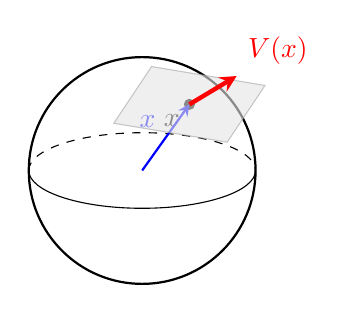
\begin{tikzpicture}[scale=1.2]
        % Esfera
        \draw[thick] (0,0) circle (1.2);
        \draw[dashed] (-1.2,0) arc (180:0:1.2 and 0.4);
        \draw (1.2,0) arc (0:-180:1.2 and 0.4);
        
        % Punto y plano tangente
        \coordinate (P) at (0.5, 0.7);
        \filldraw[black] (P) circle (1.5pt) node[below left] {$x$};
        
        % Vector normal (radio x)
        \draw[->,>=stealth,thick,blue] (0,0) -- (P) node[midway,above left] {$x$};
        
        % Plano tangente en el punto
        \draw[gray!70, fill=gray!20, opacity=0.6] (0.1, 1.1) -- (1.3, 0.9) -- (0.9, 0.3) -- (-0.3, 0.5) -- cycle;
        
        % Vector tangente V(x)
        \draw[->,>=stealth,ultra thick,red] (P) -- (1.0, 1.0) node[above right] {$V(x)$};
    \end{tikzpicture}
    \caption{Campo di vettori tangenti $V(x) \perp x$ su $S^n$.}
\end{figure}

\begin{prop}
Se esiste un campo continuo di vettori tangenti mai nullo $V: S^n \to \mathbb{R}^{n+1}$ (ossia con $V(x) \neq \bar{0}, \, \forall x \in S^n$), allora $\mathrm{Id}_{S^n} \simeq -\mathrm{Id}_{S^n}$.
\end{prop}

\begin{proof}
Poiché $V(x) \neq \bar{0}$ per ogni $x \in S^n$, possiamo definire la mappa normalizzata:
\Func{\widetilde{V}}{S^n}{S^n}{x}{\frac{V(x)}{\|V(x)\|}}
$\widetilde{V}$ è ben posta e continua. 

Osserviamo che $\widetilde{V}(x) \neq x$ per ogni $x \in S^n$. Infatti, se per assurdo esistesse $\bar{x} \in S^n$ tale che $\widetilde{V}(\bar{x}) = \bar{x}$, avremmo:
\[
1 = \langle \bar{x}, \bar{x} \rangle = \langle \widetilde{V}(\bar{x}), \bar{x} \rangle = \left\langle \frac{V(\bar{x})}{\|V(\bar{x})\|}, \bar{x} \right\rangle = \frac{1}{\|V(\bar{x})\|} \langle V(\bar{x}), \bar{x} \rangle = 0
\]
il che è una contraddizione ($1 = 0$). Pertanto $\widetilde{V}(x) \neq x$ per ogni $x \in S^n$.

Per il Corollario 1, si ha che $\widetilde{V} \simeq -\mathrm{Id}_{S^n}$.

Con un argomento analogo (dimostrando che $\widetilde{V}(x) \neq -x$ per ogni $x \in S^n$):
\[
\langle \widetilde{V}(x), x \rangle = \frac{1}{\|V(x)\|} \langle V(x), x \rangle = 0 \neq -1 = \langle -x, x \rangle
\]
si ottiene, per il Corollario 2, che $\widetilde{V} \simeq \mathrm{Id}_{S^n}$.

Dalla proprietà transitiva della relazione di omotopia segue che:
\[
\mathrm{Id}_{S^n} \simeq \widetilde{V} \simeq -\mathrm{Id}_{S^n} \implies \mathrm{Id}_{S^n} \simeq -\mathrm{Id}_{S^n}
\]
\end{proof}

\begin{prop}
Se $n$ è dispari, allora esiste un campo continuo di vettori tangenti mai nullo $V: S^n \to \mathbb{R}^{n+1}$ (ossia $V(x) \neq \bar{0}$ per ogni $x \in S^n$).
\end{prop}

\begin{proof}
Sia $n$ dispari. Allora $n = 2k-1$ per qualche $k \geqslant 1$. Identifichiamo $\mathbb{R}^{n+1} = \mathbb{R}^{2k}$ come la coppia di vettori $(x_1, \dots, x_k, y_1, \dots, y_k) \in \mathbb{R}^k \times \mathbb{R}^k$. Pertanto:
\[
S^n = S^{2k-1} = \left\{ (x_1, \dots, x_k, y_1, \dots, y_k) \in \mathbb{R}^{2k} \;\middle|\; \sum_{i=1}^k x_i^2 + \sum_{i=1}^k y_i^2 = 1 \right\}
\]
Definiamo la mappa $V: S^n \to \mathbb{R}^{2k}$ mediante:
\Func{V}{S^n}{\mathbb{R}^{2k}}{(x_1, \dots, x_k, y_1, \dots, y_k)}{(-y_1, \dots, -y_k, x_1, \dots, x_k)}

Verifichiamo le proprietà del campo di vettori:
\begin{enumerate}[label=\roman*)]
    \item $V$ è continua poiché le sue componenti sono applicazioni lineari (quindi continue) delle coordinate.
    \item $V$ è ortogonale a $x$ per ogni $x \in S^n$:
    \[
    \langle x, V(x) \rangle = \sum_{i=1}^k x_i(-y_i) + \sum_{i=1}^k y_i(x_i) = -\sum_{i=1}^k x_i y_i + \sum_{i=1}^k x_i y_i = 0
    \]
    Quindi $V$ è un campo continuo di vettori tangenti su $S^n$.
    \item La norma del campo è pari alla norma di $x$:
    \[
    \|V(x)\|^2 = \sum_{i=1}^k (-y_i)^2 + \sum_{i=1}^k x_i^2 = \sum_{i=1}^k x_i^2 + \sum_{i=1}^k y_i^2 = \|x\|^2 = 1
    \]
    Di conseguenza $\|V(x)\| = 1$, il che implica che $V(x) \neq \bar{0}$ per ogni $x \in S^n$.
\end{enumerate}
\end{proof}

\begin{figure}[H]
    \centering
    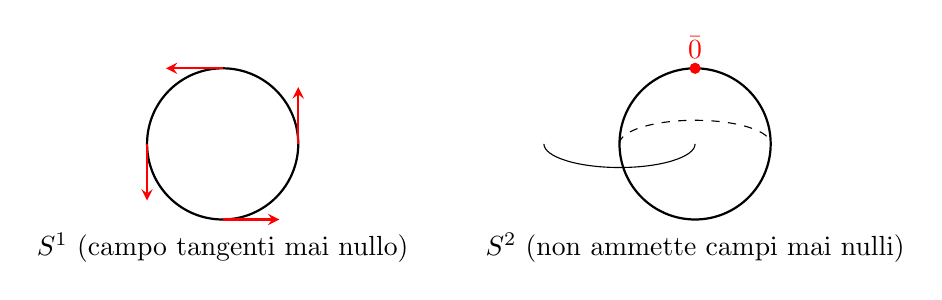
\begin{tikzpicture}[scale=1.2]
        % S^1
        \draw[thick] (-2.5,0) circle (0.8);
        \node at (-2.5, -1.1) {$S^1$ (campo tangenti mai nullo)};
        \draw[->,>=stealth,red,thick] (-2.5,0.8) -- (-3.1,0.8);
        \draw[->,>=stealth,red,thick] (-2.5,-0.8) -- (-1.9,-0.8);
        \draw[->,>=stealth,red,thick] (-3.3,0) -- (-3.3,-0.6);
        \draw[->,>=stealth,red,thick] (-1.7,0) -- (-1.7,0.6);

        % S^2
        \draw[thick] (2.5,0) circle (0.8);
        \draw[dashed] (1.7,0) arc (180:0:0.8 and 0.25);
        \draw (2.5,0) arc (0:-180:0.8 and 0.25);
        \node at (2.5, -1.1) {$S^2$ (non ammette campi mai nulli)};
        \filldraw[red] (2.5,0.8) circle (1.5pt) node[above] {$\bar{0}$};
    \end{tikzpicture}
    \caption{Visualizzazione intuitiva del Teorema del Pettine (Hairy Ball Theorem).}
\end{figure}

\begin{observacion}
Ricapitolando i risultati ottenuti sulle sfere:
\[
n \text{ è dispari} \iff \mathrm{Id}_{S^n} \simeq -\mathrm{Id}_{S^n} \iff \exists\, V \text{ campo continuo di vettori tangenti mai nullo su } S^n
\]
In particolare, se $n$ è pari, ogni campo continuo di vettori tangenti $V$ su $S^n$ ammette almeno un punto di annullamento, ovvero esiste $x \in S^n$ tale che $V(x) = \bar{0}$ (Teorema della palla pelosa).
\end{observacion}

\vspace{1.5em}

\begin{prop}
Se $n$ è pari, allora per ogni applicazione continua $f: S^n \to S^n$ esiste un punto $x_0 \in S^n$ tale che $f(x_0) = x_0$ oppure $f(x_0) = -x_0$.
\end{prop}

% Explicación en español:
% Esta proposición asegura que cualquier mapa continuo en una esfera de dimensión par tiene al menos un punto fijo o un punto antipodal fijo.

\begin{proof}
Procediamo per assurdo. Supponiamo che per ogni $x \in S^n$ si abbia $f(x) \neq x$ e $f(x) \neq -x$.

Poiché $f(x) \neq -x$ per ogni $x \in S^n$, per il Corollario 2 della sezione precedente si ha che $f \simeq \mathrm{Id}_{S^n}$.
Analogamente, poiché $f(x) \neq x$ per ogni $x \in S^n$, per il Corollario 1 si ha che $f \simeq -\mathrm{Id}_{S^n}$.

Per la proprietà di simmetria e transitività dell'omotopia, si deduce che:
\[
\mathrm{Id}_{S^n} \simeq f \simeq -\mathrm{Id}_{S^n} \implies \mathrm{Id}_{S^n} \simeq -\mathrm{Id}_{S^n}
\]
Ciò implica che $n$ debba essere dispari, in contraddizione con l'ipotesi che $n$ sia pari.
\end{proof}

\vspace{2em}

\section{Spazi omotopicamente equivalenti}

\begin{definicion}
Due spazi topologici $X$ e $Y$ si dicono \textbf{topologicamente equivalenti} (o \textbf{omeomorfi}), e si scrive $X \cong Y$, se esiste un'applicazione $f: X \to Y$ continua, invertibile e con inversa $f^{-1}: Y \to X$ continua.

Equivalentemente, esistono $f: X \to Y$ e $g: Y \to X$ continue tali che:
\[
g \circ f = \mathrm{Id}_X \quad \text{e} \quad f \circ g = \mathrm{Id}_Y
\]
In tal caso $g = f^{-1}$.
\end{definicion}

\begin{definicion}
Due spazi topologici $X$ e $Y$ si dicono \textbf{omotopicamente equivalenti} (e si scrive $X \simeq Y$) se esistono mappe continue $f: X \to Y$ e $g: Y \to X$ tali che:
\[
g \circ f \simeq \mathrm{Id}_X \quad \text{e} \quad f \circ g \simeq \mathrm{Id}_Y
\]
\end{definicion}

\begin{observacion}
La relazione di equivalenza omotopica è un indebolimento del concetto di omeomorfismo:
\[
X \cong Y \implies X \simeq Y
\]
Il viceversa non vale in generale. Ad esempio, consideriamo $X = \mathbb{R}^n$ e $Y = \{y_0\}$. Poiché $\mathbb{R}^n$ non è in biezioni con un singolo punto per $n \geqslant 1$, $\mathbb{R}^n \not\cong \{y_0\}$. Tuttavia, sono omotopicamente equivalenti ($\mathbb{R}^n \simeq \{y_0\}$).

Infatti, definiamo le applicazioni continue:
\Func{f}{\mathbb{R}^n}{\{y_0\}}{x}{y_0}
\Func{g}{\{y_0\}}{\mathbb{R}^n}{y_0}{\bar{0}}

Analizziamo le composizioni:
\begin{itemize}
    \item $(f \circ g): \{y_0\} \to \{y_0\}$ invia $y_0 \mapsto \bar{0} \mapsto y_0$, dunque $f \circ g = \mathrm{Id}_{\{y_0\}}$, che è banalmente omotopa a $\mathrm{Id}_{\{y_0\}}$.
    \item $(g \circ f): \mathbb{R}^n \to \mathbb{R}^n$ invia $x \mapsto \bar{0}$. La mappa costante $g \circ f = \bar{0}$ è omotopa a $\mathrm{Id}_{\mathbb{R}^n}$ tramite l'omotopia lineare $H(x,s) = (1-s)x$.
\end{itemize}
Dunque $\mathbb{R}^n \simeq \{y_0\}$.
\end{observacion}

\begin{teo}
L'equivalenza omotopica tra spazi topologici è una relazione di equivalenza.
\end{teo}

\begin{proof}[Dimostrazione del Teorema]
Verifichiamo le tre proprietà per dimostrare che la relazione di equivalenza omotopica $\simeq$ è una relazione di equivalenza:

\begin{itemize}
    \item \textbf{Riflessività:} Per ogni spazio topologico $X$, si ha $X \simeq X$.
    Infatti, basta considerare l'applicazione identità $\mathrm{Id}_X: X \to X$. Risulta $\mathrm{Id}_X \circ \mathrm{Id}_X = \mathrm{Id}_X \simeq \mathrm{Id}_X$, quindi la proprietà segue direttamente dalla definizione.

    \item \textbf{Simmetria:} Siano $X, Y$ spazi topologici tali che $X \simeq Y$.
    Per definizione esistono due mappe continue $f: X \to Y$ e $g: Y \to X$ tali che $g \circ f \simeq \mathrm{Id}_X$ e $f \circ g \simeq \mathrm{Id}_Y$. Scambiando i ruoli di $f$ e $g$ si ottiene immediatamente che $Y \simeq X$.

    \item \textbf{Transitività:} Siano $X, Y, Z$ spazi topologici tali che $X \simeq Y$ e $Y \simeq Z$.
    
    Per ipotesi esistono mappe continue:
    \[
    X \xleftrightarrow[g]{f} Y \quad \text{con } g \circ f \simeq \mathrm{Id}_X \text{ e } f \circ g \simeq \mathrm{Id}_Y
    \]
    \[
    Y \xleftrightarrow[g']{f'} Z \quad \text{con } g' \circ f' \simeq \mathrm{Id}_Y \text{ e } f' \circ g' \simeq \mathrm{Id}_Z
    \]
    
    Consideriamo le composizioni $f' \circ f: X \to Z$ e $g \circ g': Z \to X$. Verifichiamo le due omotopie necessarie:
    
    \begin{enumerate}[label=\roman*)]
        \item Per la composizione $(g \circ g') \circ (f' \circ f)$:
        \[
        (g \circ g') \circ (f' \circ f) = g \circ (g' \circ f') \circ f \simeq g \circ \mathrm{Id}_Y \circ f = g \circ f \simeq \mathrm{Id}_X
        \]
        \item Per la composizione $(f' \circ f) \circ (g \circ g')$:
        \[
        (f' \circ f) \circ (g \circ g') = f' \circ (f \circ g) \circ g' \simeq f' \circ \mathrm{Id}_Y \circ g' = f' \circ g' \simeq \mathrm{Id}_Z
        \]
    \end{enumerate}
    Di conseguenza $X \simeq Z$.
\end{itemize}
\end{proof}

\vspace{1.5em}

\begin{ejemplo}
Analizziamo alcuni esempi fondamentali di equivalenza omotopica:

\begin{enumerate}
    \item \textbf{Spazi convessi:} Se $\Omega \subseteq \mathbb{R}^n$ è un insieme convesso non vuoto e $x_0 \in \Omega$, allora $\Omega \simeq \{x_0\}$.
    
    % Nota en español: Todo conjunto convexo en R^n es contraíble a cualquiera de sus puntos mediante la homotopía en línea recta H(x,s) = (1-s)x + s*x_0.

    \item \textbf{Spazio euclideo privato dell'origine e la sfera $n$-dimensionale:}
    \[
    \mathbb{R}^{n+1} \setminus \{\bar{0}\} \simeq S^n
    \]
    
    Consideriamo le mappe continue:
    \Func{f}{\mathbb{R}^{n+1} \setminus \{\bar{0}\}}{S^n}{x}{\frac{x}{\|x\|} = \phi(x)}
    e l'inclusione canonica $g = i: S^n \hookrightarrow \mathbb{R}^{n+1} \setminus \{\bar{0}\}$ con $g(x) = x$.

    Analizziamo le due composizioni:
    \begin{itemize}
        \item $(g \circ f)(x) = g(\phi(x)) = \phi(x)$. Come dimostrato in precedenza, $\phi \simeq \mathrm{Id}_{\mathbb{R}^{n+1} \setminus \{\bar{0}\}}$ tramite la proiezione radicale.
        \item $(f \circ g)(x) = f(x) = \frac{x}{\|x\|} = x = \mathrm{Id}_{S^n}(x)$ per ogni $x \in S^n$ (poiché $\|x\| = 1$). Pertanto $f \circ g = \mathrm{Id}_{S^n} \simeq \mathrm{Id}_{S^n}$.
    \end{itemize}
    Dunque $\mathbb{R}^{n+1} \setminus \{\bar{0}\} \simeq S^n$.

    \item \textbf{Palla unitaria piena e il suo bordo (sfera):}
    Sia $B^n = \{x \in \mathbb{R}^n \mid \|x\| \leqslant 1\}$ la palla chiusa e $\partial B^n = \{x \in \mathbb{R}^n \mid \|x\| = 1\} = S^{n-1}$ il suo bordo.
    
    Allora, $B^{n+1} \setminus \{\bar{0}\} \simeq \partial B^{n+1} = S^n$.

    Consideriamo le mappe continue:
    \Func{f}{B^{n+1} \setminus \{\bar{0}\}}{S^n}{x}{\frac{x}{\|x\|}}
    e l'inclusione $g = i: S^n \hookrightarrow B^{n+1} \setminus \{\bar{0}\}$ dato da $g(x) = x$. Con lo stesso argomento della proiezione radicale si conclude che $B^{n+1} \setminus \{\bar{0}\} \simeq S^n$.
\end{enumerate}
\end{ejemplo}

\vspace{1.5em}

\begin{observacion}
Dalla transitività dell'equivalenza omotopica, se due spazi $X$ e $Y$ sono entrambi omotopicamente equivalenti a uno stesso spazio $Z$, allora $X \simeq Y$.

In particolare, consideriamo la sfera senza un punto: $S^n \setminus \{P\}$. Dimostreremo che $S^n \setminus \{P\} \cong \mathbb{R}^n$ e di conseguenza $S^n \setminus \{P\} \simeq \mathbb{R}^n \simeq \{x_0\}$.
\end{observacion}

\begin{prop}
La sfera $n$-dimensionale privata del Polo Nord $N = (0, \dots, 0, 1) \in \mathbb{R}^{n+1}$ è omeomorfa allo spazio euclideo $\mathbb{R}^n$:
\[
S^n \setminus \{N\} \cong \mathbb{R}^n
\]
\end{prop}

\begin{proof}
Consideriamo la \textbf{proiezione stereografica} dal Polo Nord $N = (0, \dots, 0, 1)$ sull'iperpiano $x_{n+1} = 0$, identificato con $\mathbb{R}^n$:
\Func{\varphi}{S^n \setminus \{N\}}{\mathbb{R}^n}{(x_1, \dots, x_n, x_{n+1})}{\left( \frac{x_1}{1 - x_{n+1}}, \, \dots, \, \frac{x_n}{1 - x_{n+1}} \right)}

Geometricamente, $\varphi(x)$ rappresenta l'unica intersezione dell'iperpiano $x_{n+1} = 0$ con la semiretta con origine in $N$ e passante per il punto $x \in S^n \setminus \{N\}$.

\begin{figure}[H]
    \centering
    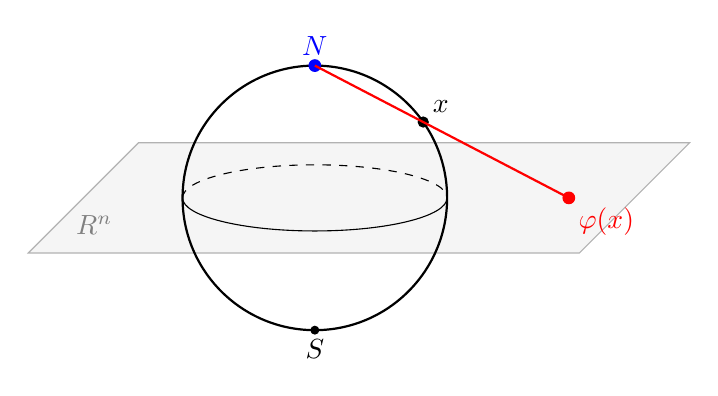
\begin{tikzpicture}[scale=1.4]
        \draw[gray!60, fill=gray!8] (-2.6,-0.5) -- (2.4,-0.5) -- (3.4,0.5) -- (-1.6,0.5) -- cycle;
        \node[gray] at (-2.0,-0.25) {$\mathbb{R}^n$};
        \draw[thick] (0,0) circle (1.2);
        \draw[dashed] (-1.2,0) arc (180:0:1.2 and 0.3);
        \draw (1.2,0) arc (0:-180:1.2 and 0.3);
        \coordinate (N) at (0,1.2);
        \filldraw[blue] (N) circle (1.5pt) node[above] {$N$};
        \coordinate (X) at (0.983,0.688);
        \filldraw (X) circle (1.3pt) node[above right] {$x$};
        \draw[red, thick] (N) -- (2.304,0);
        \filldraw[red] (2.304,0) circle (1.5pt) node[below right] {$\varphi(x)$};
        \filldraw (0,-1.2) circle (1pt) node[below] {$S$};
    \end{tikzpicture}
    \caption{Proiezione stereografica dal Polo Nord $N$ sull'iperpiano equatoriale $x_{n+1}=0$ ($\cong \mathbb{R}^n$): $\varphi(x)$ \`e l'intersezione della retta per $N$ e $x$ con l'iperpiano.}
\end{figure}

L'applicazione $\varphi$ è continua e invertibile. La sua inversa $\varphi^{-1}: \mathbb{R}^n \to S^n \setminus \{N\}$ è data da:
\Func{\varphi^{-1}}{\mathbb{R}^n}{S^n \setminus \{N\}}{(y_1, \dots, y_n)}{\left( \frac{2y_1}{\|y\|^2 + 1}, \, \dots, \, \frac{2y_n}{\|y\|^2 + 1}, \, \frac{\|y\|^2 - 1}{\|y\|^2 + 1} \right)}
dove $\|y\|^2 = y_1^2 + \dots + y_n^2$.

Poiché sia $\varphi$ che $\varphi^{-1}$ sono continue, $\varphi$ è un omeomorfismo. Pertanto $S^n \setminus \{N\} \cong \mathbb{R}^n$.
\end{proof}

\begin{observacion}
Consideriamo la proiezione stereografica dal Polo Sud $S = (0, 0, \dots, 0, -1) \in S^n$:
\[
\varphi(S) = (0, 0, \dots, 0) = \bar{0} \in \mathbb{R}^n
\]
Inoltre, l'equatore della sfera $S^n \cap \{x_{n+1} = 0\}$ equivale a $S^{n-1}$, e per ogni punto $x \in S^{n-1}$ vale $\varphi(x) = x$.

Di conseguenza:
\[
S^n \setminus \{N\} \cong \mathbb{R}^n \implies S^n \setminus \{N, S\} \cong \mathbb{R}^n \setminus \{\bar{0}\}
\]
E poiché $\mathbb{R}^n \setminus \{\bar{0}\} \simeq S^{n-1}$, si ottiene che la sfera privata dei due poli è omotopicamente equivalente alla sfera di dimensione inferiore:
\[
S^n \setminus \{N, S\} \simeq S^{n-1}
\]
\end{observacion}

\vspace{1.5em}

\section{Retratti e Retratti di Deformazione}

\begin{definicion}
Sia $Y$ uno spazio topologico e $X \subseteq Y$. $X$ si dice \textbf{retratto} di $Y$ se esiste un'applicazione continua $r: Y \to X$ tale che:
\[
r \circ i = \mathrm{Id}_X \quad (\text{cioè } r(x) = x, \; \forall x \in X)
\]
L'applicazione $r$ si dice \textbf{retrazione}.
\end{definicion}

% Nota en español: Una retracción 'r' es una proyección continua de todo el espacio Y sobre su subespacio X que deja fijos a todos los puntos de X.

\begin{ejemplo}
\begin{enumerate}
    \item Per ogni spazio topologico $Y$ e per ogni punto $y_0 \in Y$, il singoletto $\{y_0\}$ è un retratto di $Y$.
    Infatti, l'applicazione costante $r: Y \to \{y_0\}$ definita da $r(y) = y_0$ è continua e soddisfa $r(y_0) = y_0$.

    \item In generale, il fatto che $X \subseteq Y$ \textbf{non} implica che $X$ sia un retratto di $Y$.
\end{enumerate}
\end{ejemplo}

\begin{ejemplo}[Controesempio]
Sia $Y = I = [0,1]$ e $X = \mathring{I} = (0,1)$.

Supponiamo per assurdo che esista una retrazione $r: [0,1] \to (0,1)$. Allora $r$ è continua e suriettiva. Poiché $[0,1]$ è un insieme compatto e $r$ è continua, l'immagine $r([0,1]) = (0,1)$ dovrebbe essere un sottoinsieme compatto di $\mathbb{R}$. Tuttavia, l'intervallo aperto $(0,1)$ non è compatto, il che genera una contraddizione.

\textit{Nota generale:} Se $Y$ è compatto (o connesso) e $X \subseteq Y$ non è compatto (o non connesso), allora $X$ non può essere un retratto di $Y$. Ad esempio, l'interno della palla aperta $X = \mathring{B}^n$ non è un retratto della palla chiusa $Y = B^n$.
\end{ejemplo}

\begin{prop}
Siano $Y, Z$ spazi topologici, $X \subseteq Y$ ed $r: Y \to X$ una retrazione. Allora per ogni applicazione continua $f: X \to Z$, esiste un'estensione continua $\bar{f}: Y \to Z$ tale che $\bar{f}\vert_X = f$.
\end{prop}

\begin{proof}
Basta definire $\bar{f} = f \circ r: Y \to Z$. Poiché è composizione di mappe continue, $\bar{f}$ è continua, e per ogni $x \in X$ si ha $\bar{f}(x) = f(r(x)) = f(x)$.
\end{proof}

\begin{observacion}
Essere un retratto \textbf{non} implica l'equivalenza omotopica: $X$ retratto di $Y \centernot\implies X \simeq Y$.

Come controesempio, si consideri $Y = S^1$ e $X = \{x_0\} \subset S^1$. Il punto $\{x_0\}$ è un retratto di $S^1$, ma $S^1 \not\simeq \{x_0\}$ in quanto hanno gruppo fondamentale diverso ($\pi_1(S^1) \cong \mathbb{Z} \neq \{0\} = \pi_1(\{x_0\})$).

Per avere un'equivalenza omotopica occorre che $r \circ i = \mathrm{Id}_X$ e anche $i \circ r \simeq \mathrm{Id}_Y$ (retratto di deformazione).
\end{observacion}

\vspace{1.5em}

\begin{ejemplo}[Esempi di retratti di deformazione]
\begin{enumerate}
    \item In generale, un singoletto $\{y_0\}$ \textbf{non} è un retratto di deformazione di $Y$ (ad esempio $\{x_0\} \subset S^1$).
    \item $\{x_0\} \subset \mathbb{R}^n$ è un retratto di deformazione di $\mathbb{R}^n$. Più in generale, se $\Omega \subseteq \mathbb{R}^n$ è un insieme convesso, allora ogni punto $\{x_0\} \subset \Omega$ è un retratto di deformazione di $\Omega$ tramite $r(x) = x_0$.
    \item $S^n$ è un retratto di deformazione di $\mathbb{R}^{n+1} \setminus \{\bar{0}\}$ tramite la proiezione radicale:
    \Func{r}{\mathbb{R}^{n+1} \setminus \{\bar{0}\}}{S^n}{x}{\frac{x}{\|x\|}}
    \item $S^n = \partial B^{n+1} \setminus \{\bar{0}\}$ è un retratto di deformazione di $B^{n+1} \setminus \{\bar{0}\}$.
    \item Per ogni $\delta > 0$, la palla chiusa di raggio $\delta$, $B_\delta^n = \{x \in \mathbb{R}^n \mid \|x\| \leqslant \delta\}$, è un retratto di deformazione di $\mathbb{R}^n$.
\end{enumerate}
\end{ejemplo}

\begin{proof}[Dimostrazione dell'Esempio 5]
Definiamo la mappa $r: \mathbb{R}^n \to B_\delta^n$ come la proiezione radiale sulla palla:
\[
r(x) = 
\begin{cases}
    x & \text{se } \|x\| \leqslant \delta \\
    \delta \dfrac{x}{\|x\|} & \text{se } \|x\| \geqslant \delta
\end{cases}
\]

\begin{figure}[H]
    \centering
    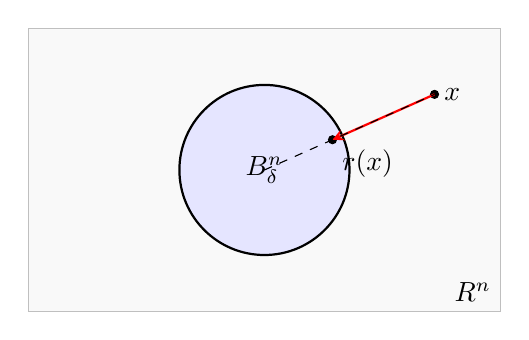
\begin{tikzpicture}[scale=1.2]
        % Plano R^n
        \draw[gray!50, fill=gray!5] (-2.5,-1.5) -- (2.5,-1.5) -- (2.5,1.5) -- (-2.5,1.5) -- cycle;
        \node[above left] at (2.5,-1.5) {$\mathbb{R}^n$};

        % Bola B_\delta^n
        \draw[thick, fill=blue!10] (0,0) circle (0.9);
        \node at (0,0) {$B_\delta^n$};

        % Puntos y proyecciones
        \filldraw (1.8,0.8) circle (1.2pt) node[right] {$x$};
        \filldraw (0.72,0.32) circle (1.2pt) node[below right] {$r(x)$};
        \draw[->,>=stealth,red,thick] (1.8,0.8) -- (0.72,0.32);

        \draw[dashed] (0,0) -- (1.8,0.8);
    \end{tikzpicture}
    \caption{Proiezione radiale di $\mathbb{R}^n$ sulla palla $B_\delta^n$.}
\end{figure}

Sulla frontiera $\|x\| = \delta$, le due definizioni coincidono: $\delta \frac{x}{\|x\|} = \delta \frac{x}{\delta} = x$. Per il \textit{Lemma di Incollamento}, $r$ è continua ed è ben posta.

Inoltre, $r(x) = x$ per ogni $x \in B_\delta^n$, e l'omotopia lineare tra $i \circ r$ e $\mathrm{Id}_{\mathbb{R}^n}$ mostra che $i \circ r \simeq \mathrm{Id}_{\mathbb{R}^n}$. Di conseguenza, $B_\delta^n$ è un retratto di deformazione di $\mathbb{R}^n$.
\end{proof}

\begin{ejemplo}
$S^{n-1}$ è un retratto di deformazione di $S^n \setminus \{N, S\}$.

\begin{figure}[H]
    \centering
    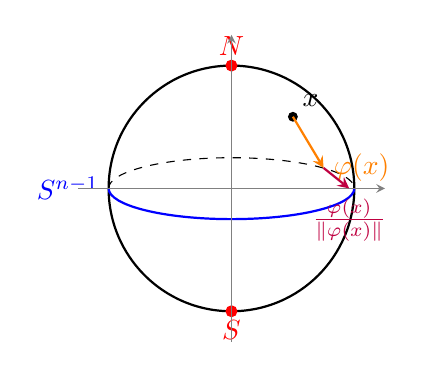
\begin{tikzpicture}[scale=1.3]
        % Esfera
        \draw[thick] (0,0) circle (1.2);
        \draw[dashed] (-1.2,0) arc (180:0:1.2 and 0.3);
        \draw[thick, blue] (1.2,0) arc (0:-180:1.2 and 0.3);
        \node[left, blue] at (-1.2, 0) {$S^{n-1}$};

        % Polos
        \filldraw[red] (0,1.2) circle (1.5pt) node[above] {$N$};
        \filldraw[red] (0,-1.2) circle (1.5pt) node[below] {$S$};

        % Ejes
        \draw[->,>=stealth,gray] (0,-1.5) -- (0,1.5);
        \draw[->,>=stealth,gray] (-1.5,0) -- (1.5,0);

        % Punto x y proyeccion
        \coordinate (X) at (0.6, 0.7);
        \filldraw (X) circle (1.2pt) node[above right] {$x$};
        
        \draw[->,>=stealth,thick,orange] (X) -- (0.9, 0.2) node[right] {$\varphi(x)$};
        \draw[->,>=stealth,thick,purple] (0.9, 0.2) -- (1.15, 0) node[below] {$\frac{\varphi(x)}{\|\varphi(x)\|}$};
    \end{tikzpicture}
    \caption{Deformazione di $S^n \setminus \{N,S\}$ su $S^{n-1}$ tramite proiezione stereografica e normalizzazione.}
\end{figure}

Geometricamente, questo si ottiene combinando la proiezione stereografica $\varphi: S^n \setminus \{N\} \to \mathbb{R}^n$, che invia $S^n \setminus \{N, S\}$ su $\mathbb{R}^n \setminus \{\bar{0}\}$, con la proiezione radicale da $\mathbb{R}^n \setminus \{\bar{0}\}$ sull'equatore $S^{n-1}$ definita da $\frac{\varphi(x)}{\|\varphi(x)\|}$.
\end{ejemplo}

\begin{proof}[Continuazione della dimostrazione]
Definiamo la mappa di retrazione:
\Func{r}{S^n \setminus \{N,S\}}{S^{n-1} = S^n \cap \{x_{n+1} = 0\}}{x}{\frac{\varphi(x)}{\|\varphi(x)\|}}

$r$ è continua e ben posta, in quanto la proiezione stereografica $\varphi$ è continua e $\varphi(x) \neq \bar{0}$ per ogni $x \in S^n \setminus \{N,S\}$.
Inoltre, per ogni $x \in S^{n-1}$, si ha $\varphi(x) = x \implies \frac{\varphi(x)}{\|\varphi(x)\|} = \frac{x}{\|x\|} = x$. Quindi $r$ è effettivamente una retrazione.

% Nota en español: Para probar que S^{n-1} es un retrato de deformación fuerte de S^n \ {N,S}, definimos la homotopía lineal normalizada entre la identidad e i o r.

Consideriamo ora la composizione $i \circ r: S^n \setminus \{N,S\} \to S^n \setminus \{N,S\}$ definita da $x \mapsto \frac{\varphi(x)}{\|\varphi(x)\|}$. Definiamo l'omotopia:
\Func{H}{(S^n \setminus \{N,S\}) \times I}{S^n \setminus \{N,S\}}{(x,s)}{\frac{(1-s)x + s\,r(x)}{\|(1-s)x + s\,r(x)\|}}

Scriviamo $x = (x', x_{n+1})$ con $x' = (x_1, \dots, x_n)$. Poich\'e $x \neq N, S$, si ha $x_{n+1} \neq \pm 1$, quindi $x' \neq \bar{0}$. Inoltre $\varphi(x) = x'/(1 - x_{n+1})$ \`e un multiplo \emph{positivo} di $x'$, per cui
\[
r(x) = \frac{\varphi(x)}{\|\varphi(x)\|} = \frac{(x', 0)}{\|x'\|} .
\]
Verifichiamo che $H$ sia ben posta e continua, ossia che il denominatore non si annulli mai:
\[
(1-s)x + s\,r(x) = \Big( \underbrace{\big(1-s + \tfrac{s}{\|x'\|}\big)}_{>0}\, x',\;\; (1-s)\,x_{n+1} \Big) \neq \bar{0}
\]
perch\'e la prima componente \`e un multiplo positivo del vettore non nullo $x'$. Inoltre il punto $H(x,s)$ ha ancora la parte orizzontale non nulla, quindi non \`e $N$ n\'e $S$: $H$ prende valori in $S^n \setminus \{N,S\}$.

Pertanto $H$ è ben posta, continua e realizza l'omotopia $\mathrm{Id}_{S^n \setminus \{N,S\}} \simeq i \circ r$. Di conseguenza, $S^{n-1}$ è un retratto di deformazione di $S^n \setminus \{N,S\}$.
\end{proof}

\vspace{1.5em}

\begin{ejemplo}
Consideriamo la sfera $S^n$ e un punto fissato $x_0 \in S^n$.
Osserviamo che l'equatore rispetto a $x_0$ è dato da:
\[
S^{n-1} = \{x \in S^n \mid \langle x, x_0 \rangle = 0\} = S^n \cap x_0^\perp
\]
Fissiamo $\varepsilon \in (0, 1)$ e definiamo la fascia equatoriale:
\[
W_\varepsilon = \{x \in S^n \mid |\langle x, x_0 \rangle| < \varepsilon\}
\]

\begin{figure}[H]
    \centering
    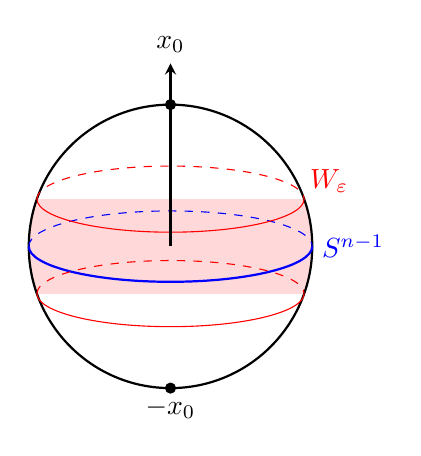
\begin{tikzpicture}[scale=1.5]
        \begin{scope}
            \clip (0,0) circle (1.2);
            \fill[red!15] (-1.3,-0.4) rectangle (1.3,0.4);
        \end{scope}
        \draw[thick] (0,0) circle (1.2);
        \draw[blue, dashed] (-1.2,0) arc (180:0:1.2 and 0.3);
        \draw[blue, thick] (-1.2,0) arc (180:360:1.2 and 0.3);
        \draw[red, dashed] (-1.131,0.4) arc (180:0:1.131 and 0.28);
        \draw[red] (-1.131,0.4) arc (180:360:1.131 and 0.28);
        \draw[red, dashed] (-1.131,-0.4) arc (180:0:1.131 and 0.28);
        \draw[red] (-1.131,-0.4) arc (180:360:1.131 and 0.28);
        \draw[->,>=stealth,thick] (0,0) -- (0,1.55) node[above] {$x_0$};
        \filldraw (0,1.2) circle (1.2pt);
        \filldraw (0,-1.2) circle (1.2pt) node[below] {$-x_0$};
        \node[blue, right] at (1.2,0) {$S^{n-1}$};
        \node[red, right] at (1.1,0.55) {$W_\varepsilon$};
    \end{tikzpicture}
    \caption{La fascia equatoriale $W_\varepsilon = \{|\langle x, x_0\rangle| < \varepsilon\}$ (in rosa) contiene l'equatore $S^{n-1}$ e non contiene i poli $\pm x_0$.}
\end{figure}

Osserviamo che:
\begin{enumerate}[label=\roman*)]
    \item $S^{n-1} = S^n \cap x_0^\perp \subset W_\varepsilon$.
    \item $|\langle \pm x_0, x_0 \rangle| = 1 > \varepsilon \implies \pm x_0 \notin W_\varepsilon$.
\end{enumerate}
Allora $S^{n-1}$ è un retratto di deformazione di $W_\varepsilon$.
\end{ejemplo}

\begin{proof}
Definiamo l'applicazione di proiezione ortogonale normalizzata:
\Func{r}{W_\varepsilon}{S^{n-1}}{x}{\frac{x - \langle x, x_0 \rangle x_0}{\|x - \langle x, x_0 \rangle x_0\|}}

\begin{figure}[H]
    \centering
    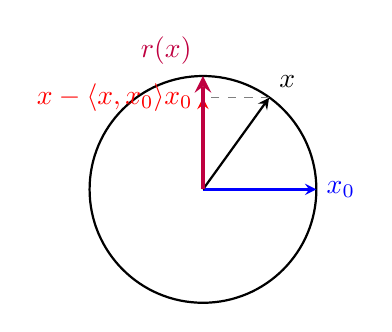
\begin{tikzpicture}[scale=1.2]
        % Circulo
        \draw[thick] (0,0) circle (1.2);
        
        % Vector x_0 y x
        \draw[->,>=stealth,thick,blue] (0,0) -- (1.2,0) node[right] {$x_0$};
        \draw[->,>=stealth,thick] (0,0) -- (0.7,0.97) node[above right] {$x$};
        
        % Proyeccion
        \draw[dashed, gray] (0.7,0.97) -- (0,0.97);
        \draw[->,>=stealth,thick,red] (0,0) -- (0,0.97) node[left] {$x - \langle x, x_0 \rangle x_0$};
        \draw[->,>=stealth,ultra thick,purple] (0,0) -- (0,1.2) node[above left] {$r(x)$};
    \end{tikzpicture}
    \caption{Proiezione ortogonale di $x$ sull'equatore $S^{n-1}$.}
\end{figure}

Verifichiamo le proprietà:
\begin{enumerate}[label=\roman*)]
    \item Il denominatore non si annulla mai in $W_\varepsilon$: infatti, $x - \langle x, x_0 \rangle x_0 = \bar{0} \implies x = \langle x, x_0 \rangle x_0 \implies x \mathbin{\|} x_0 \implies x = \pm x_0$. Tuttavia, $\pm x_0 \notin W_\varepsilon$, quindi il denominatore è sempre strettamente positivo e $r$ è continua e ben posta.
    \item $r(x) \in S^{n-1}$, in quanto:
    \[
    \langle r(x), x_0 \rangle = \frac{1}{\|x - \langle x, x_0 \rangle x_0\|} \Big( \langle x, x_0 \rangle - \langle x, x_0 \rangle \underbrace{\langle x_0, x_0 \rangle}_{=1} \Big) = 0
    \]
    \item Per ogni $x \in S^{n-1}$, vale $\langle x, x_0 \rangle = 0$, quindi $r(x) = \frac{x}{\|x\|} = x$. Dunque $r$ è una retrazione.
\end{enumerate}

Mostriamo che $i \circ r \simeq \mathrm{Id}_{W_\varepsilon}$ tramite l'omotopia lineare normalizzata:
\Func{H}{W_\varepsilon \times I}{W_\varepsilon}{(x,s)}{\frac{(1-s)x + s\,r(x)}{\|(1-s)x + s\,r(x)\|}}

Scriviamo $a = \langle x, x_0 \rangle$, con $|a| < \varepsilon < 1$, e $b = \sqrt{1-a^2} > 0$. Allora
\[
x = a\,x_0 + b\,r(x), \qquad r(x) \perp x_0, \ \|r(x)\| = 1 ,
\]
e quindi
\[
v := (1-s)x + s\,r(x) = (1-s)a\,x_0 + \big( (1-s)b + s \big)\, r(x).
\]
Poich\'e $x_0 \perp r(x)$ e $(1-s)b + s > 0$ (perch\'e $b>0$), si ha $v \neq \bar{0}$: $H$ \`e ben posta e continua.

$H$ prende valori in $W_\varepsilon$: dalla formula,
$\|v\|^2 = (1-s)^2 a^2 + \big((1-s)b + s\big)^2 \geqslant (1-s)^2 (a^2 + b^2) = (1-s)^2$, quindi
\[
|\langle H(x,s), x_0 \rangle| = \frac{(1-s)\,|a|}{\|v\|} \leqslant |a| < \varepsilon .
\]
Inoltre $H$ lascia fisso ogni punto di $S^{n-1}$ (l\`\i\ $a=0$ e $r(x)=x$).

Le verifiche ai bordi confermano che:
\begin{itemize}
    \item $H(x,0) = \frac{x}{\|x\|} = x = \mathrm{Id}_{W_\varepsilon}(x)$.
    \item $H(x,1) = \frac{r(x)}{\|r(x)\|} = r(x) = (i \circ r)(x)$.
\end{itemize}
Di conseguenza $\mathrm{Id}_{W_\varepsilon} \simeq i \circ r$, dimostrando che $S^{n-1}$ è un retratto di deformazione di $W_\varepsilon$.
\end{proof}

\vspace{2em}

\section{Spazi Contraibili}

\begin{definicion}
Uno spazio topologico $Y$ si dice \textbf{contraibile} a un suo punto $y_0 \in Y$ se l'applicazione identità $\mathrm{Id}_Y$ è omotopa alla mappa costante $c_{y_0}: Y \to Y$ (definita da $c_{y_0}(y) = y_0$ per ogni $y \in Y$):
\[
\mathrm{Id}_Y \simeq c_{y_0}
\]
\end{definicion}

% Nota en español: Un espacio contraíble es aquel que se puede deformar de manera continua hasta reducirse a un único punto.

\begin{teo}
Uno spazio topologico $Y$ è contraibile a un punto $y_0 \in Y$ se e solo se per ogni spazio topologico $X$, due qualsiasi mappe continue $f, g: X \to Y$ sono omotope ($f \simeq g$).
\end{teo}

\begin{proof}[Dimostrazione del Teorema sulla Contraibilità]
\begin{itemize}
    \item[$\impliedby$)] Banale. Basta scegliere $X = Y$ e prendere $f = \mathrm{Id}_Y$ e $g = c_{y_0}$.
    \item[$\implies$)] Siano $X$ uno spazio topologico e $f, g: X \to Y$ due mappe continue qualsiasi.
    
    Poiché $Y$ è contraibile a $y_0$, si ha $c_{y_0} \simeq \mathrm{Id}_Y$. Applicando la proprietà di composizione dell'omotopia:
    \[
    f \simeq f \quad \text{e} \quad c_{y_0} \simeq \mathrm{Id}_Y \implies c_{y_0} \circ f \simeq \mathrm{Id}_Y \circ f = f
    \]
    \[
    g \simeq g \quad \text{e} \quad c_{y_0} \simeq \mathrm{Id}_Y \implies c_{y_0} \circ g \simeq \mathrm{Id}_Y \circ g = g
    \]
    
    Osserviamo che per ogni $x \in X$:
    \[
    (c_{y_0} \circ f)(x) = c_{y_0}(f(x)) = y_0 \quad \text{e} \quad (c_{y_0} \circ g)(x) = c_{y_0}(g(x)) = y_0
    \]
    Quindi $c_{y_0} \circ f = c_{y_0} \circ g = c_{y_0}$ (la mappa costante da $X$ in $Y$ che invia tutto in $y_0$). Per transitività e simmetria:
    \[
    f \simeq c_{y_0} \circ f = c_{y_0} \circ g \simeq g \implies f \simeq g
    \]
\end{itemize}
\end{proof}

\begin{coro}
Se $Y$ è contraibile a un punto $y_0 \in Y$, allora $Y$ è contraibile a ogni suo punto $y \in Y$ (ovvero $c_y \simeq \mathrm{Id}_Y, \, \forall y \in Y$).
\end{coro}
\begin{proof}
Per il teorema, due qualsiasi mappe continue $X \to Y$ sono omotope; in particolare (con $X = Y$) $c_y \simeq \mathrm{Id}_Y$.
\end{proof}

\begin{coro}
Se $Y$ è contraibile, allora $Y$ è connesso per archi.
\end{coro}
\begin{proof}
Per il corollario precedente $c_{y_0} \simeq c_{y}$ per ogni $y \in Y$ (come mappe $Y \to Y$). Per l'esercizio sulle mappe costanti, esiste un cammino da $y_0$ a $y$. Quindi ogni punto si collega a $y_0$.
\end{proof}

\begin{observacion}
Il viceversa del Corollario 2 \textbf{non} vale in generale: connesso per archi $\centernot\implies$ contraibile.

Come controesempio, per ogni $n$ pari, la sfera $S^n$ è connessa per archi, ma la mappa identità $\mathrm{Id}_{S^n}$ non è omotopa a $-\mathrm{Id}_{S^n}$ (e quindi la sfera non è contraibile, $S^n \not\simeq \{x_0\}$).
\end{observacion}

\vspace{1.5em}

\begin{teo}
Per uno spazio topologico $Y$, le seguenti affermazioni sono equivalenti:
\begin{enumerate}
    \item $Y$ è contraibile.
    \item $Y$ ammette un suo punto $y_0$ come retratto di deformazione.
    \item $Y$ è omotopicamente equivalente a un punto (singoletto).
\end{enumerate}
\end{teo}

\begin{proof}
\begin{itemize}
    \item[$(1) \implies (2)$:] Sia $y_0 \in Y$. Per ipotesi, $c_{y_0} \simeq \mathrm{Id}_Y$.
    Sia $r: Y \to \{y_0\}$ l'unica retrazione $r(y) = y_0$. Si ha $r \circ i = \mathrm{Id}_{\{y_0\}}$.
    Inoltre, $(i \circ r)(y) = i(y_0) = y_0 = c_{y_0}(y)$. Poiché $c_{y_0} \simeq \mathrm{Id}_Y$, segue che $i \circ r \simeq \mathrm{Id}_Y$.
    Quindi $\{y_0\}$ è un retratto di deformazione di $Y$.

    \item[$(2) \implies (3)$:] Segue direttamente dalla definizione di retratto di deformazione (che fornisce un'equivalenza omotopica con il sottoinsieme $\{y_0\}$).

    \item[$(3) \implies (1)$:] Se $Y \simeq \{*\}$, esistono mappe $f: Y \to \{*\}$ e $g: \{*\} \to Y$ con $g \circ f \simeq \mathrm{Id}_Y$. Posto $y_1 = g(*)$, si ha $(g \circ f)(y) = y_1 = c_{y_1}(y)$, quindi $c_{y_1} \simeq \mathrm{Id}_Y$: $Y$ è contraibile a $y_1$, e dunque (corollario precedente) a ogni suo punto.
\end{itemize}
\end{proof}

\vspace{1.5em}

\begin{ejemplo}
\begin{enumerate}
    \item $\mathbb{R}^n$ e qualsiasi insieme convesso $\Omega \subseteq \mathbb{R}^n$ sono contraibili.
    
    \item \textbf{Insiemi stellati:} Ricordiamo che un sottoinsieme $S \subseteq \mathbb{R}^n$ si dice \textbf{stellato rispetto a un punto} $x_0 \in S$ se per ogni $x \in S$ il segmento $\overline{x\, x_0}$ è interamente contenuto in $S$:
    \[
    \overline{x\, x_0} = \{(1-s)x + s\,x_0 \mid s \in [0,1]\} \subseteq S
    \]

    \begin{figure}[H]
        \centering
        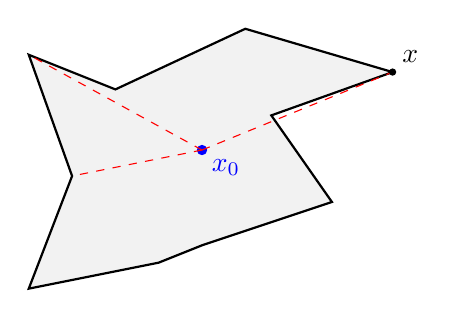
\begin{tikzpicture}[scale=1.1]
            % Dominio estrellado
            \draw[thick, fill=gray!10] 
                (0,0) -- (1.5,0.5) -- (0.8,1.5) -- (2.2,2.0) -- (0.5,2.5) 
                -- (-1,1.8) -- (-2,2.2) -- (-1.5,0.8) -- (-2,-0.5) -- (-0.5,-0.2) -- cycle;
            
            % Punto centro x_0
            \coordinate (X0) at (0, 1.1);
            \filldraw[blue] (X0) circle (1.5pt) node[below right] {$x_0$};

            % Puntos en la frontera y segmentos
            \coordinate (P1) at (2.2, 2.0);
            \coordinate (P2) at (-2, 2.2);
            \coordinate (P3) at (-1.5, 0.8);

            \draw[dashed, red] (X0) -- (P1);
            \draw[dashed, red] (X0) -- (P2);
            \draw[dashed, red] (X0) -- (P3);

            \filldraw (P1) circle (1pt) node[above right] {$x$};
        \end{tikzpicture}
        \caption{Insieme $S \subset \mathbb{R}^n$ stellato rispetto a $x_0$.}
    \end{figure}

    \begin{prop}
    Se $S \subseteq \mathbb{R}^n$ è stellato rispetto a $x_0$, allora $S$ è contraibile.
    \end{prop}

    \begin{proof}
    Definiamo la retrazione $r: S \to \{x_0\}$ con $r(x) = x_0$.
    Mostriamo che $i \circ r \simeq \mathrm{Id}_S$ tramite l'omotopia lineare:
    \Func{H}{S \times I}{S}{(x,s)}{(1-s)x + s\,x_0}
    
    Poiché $S$ è stellato rispetto a $x_0$, $H(x,s) \in S$ per ogni $x \in S$ e $s \in I$. Inoltre $H(x,0) = x$ e $H(x,1) = x_0$. Dunque $\{x_0\}$ è un retratto di deformazione di $S$, e quindi $S$ è contraibile a $x_0$.
    \end{proof}
\end{enumerate}
\end{ejemplo}

\begin{prop}
Se $X$ e $Y$ sono spazi topologici contraibili, allora il loro prodotto cartesiano $X \times Y$ è contraibile.
\end{prop}

\begin{proof}
Siano $x_0 \in X$ e $y_0 \in Y$ i punti rispetto a cui $X$ e $Y$ si contraggono.
Per ipotesi, esistono le omotopie $H: c_{x_0} \simeq \mathrm{Id}_X$ su $X \times I$ e $K: c_{y_0} \simeq \mathrm{Id}_Y$ su $Y \times I$.

Definiamo la mappa prodotto per l'omotopia:
\Func{W}{(X \times Y) \times I}{X \times Y}{\big((x,y), s\big)}{\big(H(x,s), K(y,s)\big)}

$W$ è continua in quanto le sue componenti $H$ e $K$ sono continue. Verifichiamo le condizioni agli estremi:
\begin{enumerate}[label=\roman*)]
    \item $W((x,y), 0) = (H(x,0), K(y,0)) = (x_0, y_0) = c_{(x_0,y_0)}(x,y)$.
    \item $W((x,y), 1) = (H(x,1), K(y,1)) = (x,y) = \mathrm{Id}_{X \times Y}(x,y)$.
\end{enumerate}
Pertanto $W: c_{(x_0,y_0)} \simeq \mathrm{Id}_{X \times Y}$, ovvero $X \times Y$ è contraibile.
\end{proof}

\begin{ejemplo}
Se $S \subset \mathbb{R}^n$ è un insieme stellato e $\Omega \subset \mathbb{R}^m$ è convesso, il cilindro/prodotto $S \times \Omega$ è uno spazio contraibile.
\end{ejemplo}

\begin{prop}
Siano $X, Y$ spazi topologici. Se $Y$ è contraibile, allora $X \times Y \simeq X$.
\end{prop}

\begin{proof}
Sia $y_0 \in Y$ tale che $c_{y_0} \simeq \mathrm{Id}_Y$ tramite l'omotopia $H: Y \times I \to Y$.
Consideriamo le proiezioni e inclusioni continue:
\Func{f}{X \times Y}{X}{(x,y)}{x}
\Func{g}{X}{X \times Y}{x}{(x, y_0)}

Analizziamo le due composizioni:
\begin{itemize}
    \item $(f \circ g)(x) = f(x, y_0) = x = \mathrm{Id}_X(x)$, quindi $f \circ g = \mathrm{Id}_X \simeq \mathrm{Id}_X$.
    \item $(g \circ f)(x,y) = g(x) = (x, y_0)$. Mostriamo che $g \circ f \simeq \mathrm{Id}_{X \times Y}$ costruendo l'omotopia:
    \Func{K}{(X \times Y) \times I}{X \times Y}{\big((x,y), s\big)}{\big(x, H(y,s)\big)}
    $K$ è continua e verifica $K((x,y),0) = (x, y_0) = (g \circ f)(x,y)$ e $K((x,y),1) = (x, y) = \mathrm{Id}_{X \times Y}(x,y)$.
\end{itemize}
Di conseguenza $X \times Y \simeq X$.
\end{proof}

\section{Gruppo Fondamentale e Omotopia di Cammini}

Un \textbf{cappio} (o cammino chiuso) in $X$ con punto base $x_0$ \`e un cammino $\sigma: I \to X$ con $\sigma(0) = \sigma(1) = x_0$. Indichiamo con $\Lambda_{x_0} = \Lambda_{x_0}(X)$ l'insieme dei cappi in $x_0$. La relazione di omotopia relativamente al bordo $\partial I = \{0,1\}$ \`e una relazione di equivalenza su $\Lambda_{x_0}$ (riflessiva, simmetrica e transitiva: si compongono/invertono le omotopie). Poniamo:
\[
\Pi_1(X, x_0) = \Lambda_{x_0} \big/ \!\simeq \text{ rel } \partial I
\]
Gli elementi di $\Pi_1(X, x_0)$ sono le classi di omotopia dei cammini chiusi in $X$ con base in $x_0$, relativamente a $\partial I$.

\begin{figure}[H]
    \centering
    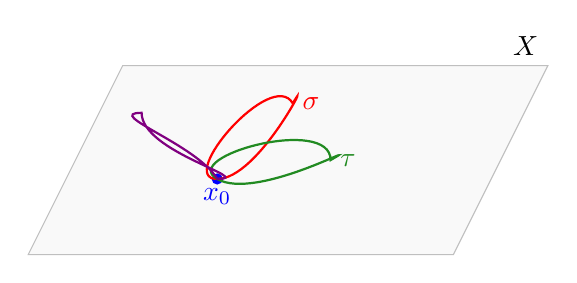
\begin{tikzpicture}[scale=1.2]
        % Plano X
        \draw[gray!50, fill=gray!5] (-2,-1) -- (2.5,-1) -- (3.5,1) -- (-1,1) -- cycle;
        \node[above left] at (3.5,1) {$X$};

        % Punto base x_0
        \coordinate (X0) at (0,-0.2);
        \filldraw[blue] (X0) circle (1.5pt) node[below] {$x_0$};

        % Lazos
        \draw[thick, red] (X0) to[out=0, in=60] (0.8, 0.6) to[out=120, in=180] (X0);
        \node[red, right] at (0.8, 0.6) {$\sigma$};

        \draw[thick, ForestGreen] (X0) to[out=-30, in=30] (1.2, 0) to[out=90, in=150] (X0);
        \node[ForestGreen, right] at (1.2, 0) {$\tau$};

        \draw[thick, Purple] (X0) to[out=120, in=180] (-0.8, 0.5) to[out=-90, in=0] (X0);
    \end{tikzpicture}
    \caption{Cappi in $X$ con punto base $x_0$.}
\end{figure}

Per ogni $\sigma \in \Lambda_{x_0}$, la classe di omotopia è indicata con:
\[
[\sigma] = \{ \tau \in \Lambda_{x_0} \mid \sigma \simeq \tau \text{ rel } \partial I \}
\]

\begin{observacion}
Siano $\sigma, \tau \in \Lambda_{x_0}$, ovvero $\sigma(1) = \tau(0) = x_0$.
Si ha che la concatenazione $\sigma * \tau \in \Lambda_{x_0}$, l'inverso $\sigma^{-1} \in \Lambda_{x_0}$ e il cammino costante $c_{x_0} \in \Lambda_{x_0}$.
\end{observacion}

\vspace{1.5em}

\begin{teo}
Sia $X$ uno spazio topologico.
\begin{enumerate}[label=\alph*)]
    \item \textbf{Compatibilità dell'omotopia rel $\partial I$ con l'operazione di concatenazione $*$:}
    Siano $\alpha, \beta, \alpha', \beta'$ cammini in $X$ tali che $\alpha(1) = \beta(0)$ e $\alpha'(1) = \beta'(0)$.
    Se $\alpha \simeq \alpha' \text{ rel } \partial I$ e $\beta \simeq \beta' \text{ rel } \partial I$, allora:
    \[
    \alpha * \beta \simeq \alpha' * \beta' \text{ rel } \partial I
    \]

    \item \textbf{Associatività a meno di omotopia:}
    Siano $\alpha, \beta, \gamma$ cammini in $X$ con $\alpha(1) = \beta(0)$ e $\beta(1) = \gamma(0)$. Allora:
    \[
    (\alpha * \beta) * \gamma \simeq \alpha * (\beta * \gamma) \text{ rel } \partial I
    \]

    \item \textbf{Elemento neutro a meno di omotopia:}
    Per ogni cammino $\alpha$ in $X$ con $\alpha(0) = x_0$ e $\alpha(1) = x_1$:
    \[
    c_{x_0} * \alpha \simeq \alpha \text{ rel } \partial I \quad \text{e} \quad \alpha * c_{x_1} \simeq \alpha \text{ rel } \partial I
    \]

    \item \textbf{Elemento inverso a meno di omotopia:}
    Per ogni cammino $\alpha$ in $X$ con $\alpha(0) = x_0$ e $\alpha(1) = x_1$:
    \[
    \alpha * \alpha^{-1} \simeq c_{x_0} \text{ rel } \partial I \quad \text{e} \quad \alpha^{-1} * \alpha \simeq c_{x_1} \text{ rel } \partial I
    \]
\end{enumerate}
\end{teo}

\begin{proof}
Dimostriamo le varie parti del teorema:

\textbf{Dimostrazione di a):}
Siano $H: \alpha \simeq \alpha' \text{ rel } \partial I$ e $K: \beta \simeq \beta' \text{ rel } \partial I$ le due omotopie relative al bordo. Definiamo la mappa $W: I \times I \to X$:
\[
W(t,s) = 
\begin{cases}
    H(2t, s) & t \leqslant \frac{1}{2} \\
    K(2t-1, s) & t \geqslant \frac{1}{2}
\end{cases}
\]

Verifichiamo la continuità e ben posizione per $t = \frac{1}{2}$:
\[
H(2 \cdot \tfrac{1}{2}, s) = H(1, s) = \alpha(1) = \beta(0) = K(0, s) = K(2 \cdot \tfrac{1}{2} - 1, s)
\]
Quindi $W$ è ben definita e continua per il Lemma di Incollamento.

Verifichiamo le condizioni ai bordi:
\begin{enumerate}[label=\roman*)]
    \item Per $s = 0$:
    \[
    W(t,0) = 
    \begin{cases}
        H(2t,0) = \alpha(2t) & t \leqslant \frac{1}{2} \\
        K(2t-1,0) = \beta(2t-1) & t \geqslant \frac{1}{2}
    \end{cases}
    = (\alpha * \beta)(t)
    \]
    \item Per $s = 1$:
    \[
    W(t,1) = 
    \begin{cases}
        H(2t,1) = \alpha'(2t) & t \leqslant \frac{1}{2} \\
        K(2t-1,1) = \beta'(2t-1) & t \geqslant \frac{1}{2}
    \end{cases}
    = (\alpha' * \beta')(t)
    \]
    \item Per $t = 0$ e $t = 1$, poiché $H$ e $K$ sono omotopie relative a $\partial I$:
    \[
    W(0,s) = H(0,s) = \alpha(0) = (\alpha * \beta)(0)
    \]
    \[
    W(1,s) = K(1,s) = \beta(1) = (\alpha * \beta)(1)
    \]
\end{enumerate}
Dunque $W: \alpha * \beta \simeq \alpha' * \beta' \text{ rel } \partial I$.

\vspace{1em}

\textbf{Dimostrazione di b) (Associatività):}
Calcoliamo le definizioni esplicite delle due riparametrizzazioni dei cammini:
\[
((\alpha * \beta) * \gamma)(t) = 
\begin{cases}
    (\alpha * \beta)(2t) = \alpha(4t) & 0 \leqslant t \leqslant \frac{1}{4} \\
    (\alpha * \beta)(2t) = \beta(4t-1) & \frac{1}{4} \leqslant t \leqslant \frac{1}{2} \\
    \gamma(2t-1) & \frac{1}{2} \leqslant t \leqslant 1
\end{cases}
\]
e
\[
(\alpha * (\beta * \gamma))(t) = 
\begin{cases}
    \alpha(2t) & 0 \leqslant t \leqslant \frac{1}{2} \\
    (\beta * \gamma)(2t-1) = \beta(4t-2) & \frac{1}{2} \leqslant t \leqslant \frac{3}{4} \\
    (\beta * \gamma)(2t-1) = \gamma(4t-3) & \frac{3}{4} \leqslant t \leqslant 1
\end{cases}
\]

Per costruire l'omotopia $H: I \times I \to X$ tra le due riparametrizzazioni, suddividiamo il quadrato $I \times I$ mediante due rette nel piano $(t,s)$:
la retta che unisce $(\frac{1}{4},0)$ a $(\frac{1}{2},1)$, di equazione $s = 4t-1$, e la retta che unisce $(\frac{1}{2},0)$ a $(\frac{3}{4},1)$, di equazione $s = 4t-2$.

\begin{figure}[H]
    \centering
    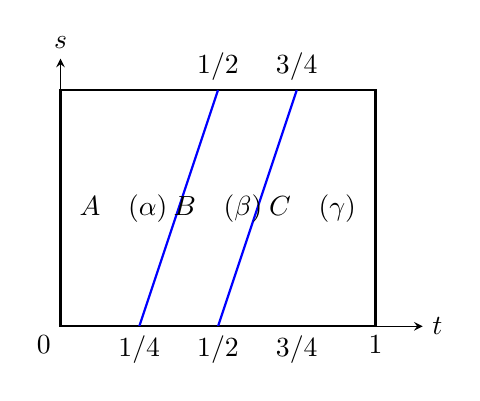
\begin{tikzpicture}[scale=2]
        % Cuadrado I x I
        \draw[thick] (0,0) -- (2,0) -- (2,1.5) -- (0,1.5) -- cycle;
        \node[below left] at (0,0) {$0$};
        \node[below] at (0.5,0) {$1/4$};
        \node[below] at (1,0) {$1/2$};
        \node[below] at (1.5,0) {$3/4$};
        \node[below] at (2,0) {$1$};

        \node[above] at (1,1.5) {$1/2$};
        \node[above] at (1.5,1.5) {$3/4$};

        % Divisiones
        \draw[thick, blue] (0.5,0) -- (1,1.5);
        \draw[thick, blue] (1,0) -- (1.5,1.5);

        % Regiones
        \node at (0.4, 0.75) {$A \quad (\alpha)$};
        \node at (1.0, 0.75) {$B \quad (\beta)$};
        \node at (1.6, 0.75) {$C \quad (\gamma)$};

        % Ejes
        \draw[->,>=stealth] (0,0) -- (2.3,0) node[right] {$t$};
        \draw[->,>=stealth] (0,0) -- (0,1.7) node[above] {$s$};
    \end{tikzpicture}
    \caption{Suddivisione del quadrato $I \times I$ per l'omotopia di associatività.}
\end{figure}

Definiamo le tre regioni del quadrato $I \times I$:
\[
A = \{ (t,s) \in I \times I \mid s \geqslant 4t-1 \}
\]
\[
B = \{ (t,s) \in I \times I \mid 4t-2 \leqslant s \leqslant 4t-1 \}
\]
\[
C = \{ (t,s) \in I \times I \mid s \leqslant 4t-2 \}
\]

Definiamo l'omotopia $H: I \times I \to X$ sulle tre regioni:
\[
H(t,s) = 
\begin{cases}
    \alpha\left( \dfrac{4t}{s+1} \right) & (t,s) \in A \\[1em]
    \beta(4t - s - 1) & (t,s) \in B \\[1em]
    \gamma\left( \dfrac{4t - s - 2}{2 - s} \right) & (t,s) \in C
\end{cases}
\]

Verifichiamo la continuità sulle linee di separazione (Lemma di Incollamento):
\begin{itemize}
    \item Sulla retta $s = 4t-1$ (confine tra $A$ e $B$):
    \[
    \alpha\left(\frac{4t}{(4t-1)+1}\right) = \alpha(1) = \beta(0) = \beta(4t - (4t-1) - 1)
    \]
    \item Sulla retta $s = 4t-2$ (confine tra $B$ e $C$):
    \[
    \beta(4t - (4t-2) - 1) = \beta(1) = \gamma(0) = \gamma\left(\frac{4t - (4t-2) - 2}{2 - (4t-2)}\right)
    \]
\end{itemize}

Controlliamo le condizioni per $s = 0$ e $s = 1$:
\begin{itemize}
    \item Per $s = 0$, le regioni corrispondono a $t \leqslant 1/4$, $1/4 \leqslant t \leqslant 1/2$ e $t \geqslant 1/2$:
    \[
    H(t,0) = 
    \begin{cases}
        \alpha(4t) & t \leqslant 1/4 \\
        \beta(4t-1) & 1/4 \leqslant t \leqslant 1/2 \\
        \gamma(2t-1) & t \geqslant 1/2
    \end{cases}
    = ((\alpha * \beta) * \gamma)(t)
    \]
    \item Per $s = 1$, le regioni corrispondono a $t \leqslant 1/2$, $1/2 \leqslant t \leqslant 3/4$ e $t \geqslant 3/4$:
    \[
    H(t,1) = 
    \begin{cases}
        \alpha(2t) & t \leqslant 1/2 \\
        \beta(4t-2) & 1/2 \leqslant t \leqslant 3/4 \\
        \gamma(4t-3) & t \geqslant 3/4
    \end{cases}
    = (\alpha * (\beta * \gamma))(t)
    \]
\end{itemize}
Inoltre $H(0,s) = \alpha(0)$ e $H(1,s) = \gamma(1)$ per ogni $s \in I$.
Pertanto $H$ è continua e dimostra l'associatività a meno di omotopia: $(\alpha * \beta) * \gamma \simeq \alpha * (\beta * \gamma) \text{ rel } \partial I$.
\end{proof}

\textbf{Dimostrazione di c) (Elemento neutro):}
Dimostriamo che $c_{x_0} * \alpha \simeq \alpha \text{ rel } \partial I$ (la dimostrazione per $\alpha * c_{x_1} \simeq \alpha$ è del tutto analoga).

Consideriamo la retta nel piano $(t,s)$ che unisce i punti $(\frac{1}{2}, 0)$ e $(1,1)$, avente equazione $s = 2t - 1$.

\begin{figure}[H]
    \centering
    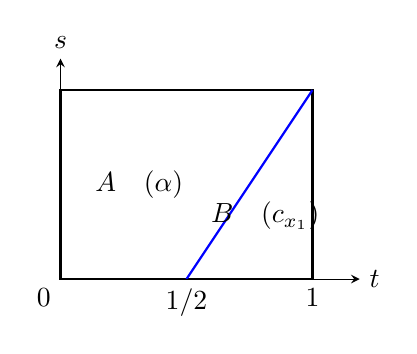
\begin{tikzpicture}[scale=2]
        % Cuadrado I x I
        \draw[thick] (0,0) -- (1.6,0) -- (1.6,1.2) -- (0,1.2) -- cycle;
        \node[below left] at (0,0) {$0$};
        \node[below] at (0.8,0) {$1/2$};
        \node[below] at (1.6,0) {$1$};

        % Linea de separación s = 2t - 1
        \draw[thick, blue] (0.8,0) -- (1.6,1.2);

        % Regiones A y B
        \node at (0.5, 0.6) {$A \quad (\alpha)$};
        \node at (1.3, 0.4) {$B \quad (c_{x_1})$};

        % Ejes
        \draw[->,>=stealth] (0,0) -- (1.9,0) node[right] {$t$};
        \draw[->,>=stealth] (0,0) -- (0,1.4) node[above] {$s$};
    \end{tikzpicture}
    \caption{Divisione del quadrato $I \times I$ per l'omotopia dell'elemento neutro.}
\end{figure}

Definiamo le regioni $A$ e $B$:
\[
A = \{ (t,s) \in I \times I \mid s \geqslant 2t - 1 \}
\]
\[
B = \{ (t,s) \in I \times I \mid s \leqslant 2t - 1 \}
\]

Definiamo l'omotopia $H: I \times I \to X$:
\[
H(t,s) = 
\begin{cases}
    \alpha\left( \dfrac{2t}{s+1} \right) & (t,s) \in A \\[1em]
    x_1 & (t,s) \in B
\end{cases}
\]

Verifichiamo la continuità sulla linea di giunzione $s = 2t - 1$ ($2t = s + 1$):
\[
\alpha\left( \frac{2t}{s+1} \right) = \alpha(1) = x_1
\]
Per il Lemma di Incollamento, $H$ è ben posta e continua.

Verifichiamo le condizioni ai bordi:
\begin{enumerate}[label=\roman*)]
    \item Per $s = 0$:
    \[
    H(t,0) = 
    \begin{cases}
        \alpha(2t) & t \leqslant \frac{1}{2} \\
        x_1 & t \geqslant \frac{1}{2}
    \end{cases}
    = (\alpha * c_{x_1})(t)
    \]
    \item Per $s = 1$:
    \[
    H(t,1) = \alpha\left( \frac{2t}{2} \right) = \alpha(t)
    \]
    \item Per $t = 0$ e $t = 1$:
    \[
    H(0,s) = \alpha(0) = x_0 \quad \text{e} \quad H(1,s) = x_1
    \]
\end{enumerate}
Quindi $H: \alpha * c_{x_1} \simeq \alpha \text{ rel } \partial I$.

\vspace{1.5em}

\textbf{Dimostrazione di d) (Elemento inverso):}
Dimostriamo che $\alpha * \alpha^{-1} \simeq c_{x_0} \text{ rel } \partial I$.

Consideriamo le rette $s = 2t$ (tra $(0,0)$ e $(\frac{1}{2},1)$) e $s = 2 - 2t$ (tra $(\frac{1}{2},1)$ e $(1,0)$).

\begin{figure}[H]
    \centering
    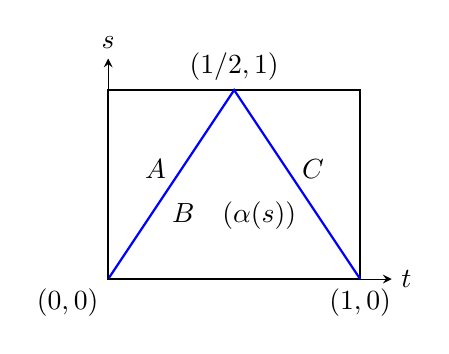
\begin{tikzpicture}[scale=2]
        % Cuadrado I x I
        \draw[thick] (0,0) -- (1.6,0) -- (1.6,1.2) -- (0,1.2) -- cycle;
        \node[below left] at (0,0) {$(0,0)$};
        \node[below] at (1.6,0) {$(1,0)$};
        \node[above] at (0.8,1.2) {$(1/2,1)$};

        % Triangulo interior B
        \draw[thick, blue] (0,0) -- (0.8,1.2) -- (1.6,0);

        % Regiones
        \node at (0.3, 0.7) {$A$};
        \node at (0.8, 0.4) {$B \quad (\alpha(s))$};
        \node at (1.3, 0.7) {$C$};

        % Ejes
        \draw[->,>=stealth] (0,0) -- (1.8,0) node[right] {$t$};
        \draw[->,>=stealth] (0,0) -- (0,1.4) node[above] {$s$};
    \end{tikzpicture}
    \caption{Suddivisione per l'omotopia dell'elemento inverso.}
\end{figure}

Definiamo le regioni del quadrato:
\[
A = \{ (t,s) \in I \times I \mid 2t \leqslant s \}
\]
\[
B = \{ (t,s) \in I \times I \mid s \leqslant 2t \text{ e } s \leqslant 2 - 2t \}
\]
\[
C = \{ (t,s) \in I \times I \mid 2t \geqslant 2 - s \}
\]

Definiamo l'omotopia $H: I \times I \to X$:
\[
H(t,s) = 
\begin{cases}
    \alpha(2t) & (t,s) \in A \\
    \alpha(s) & (t,s) \in B \\
    \alpha^{-1}(2t-1) = \alpha(2 - 2t) & (t,s) \in C
\end{cases}
\]

Sui confini della regione $B$:
\begin{itemize}
    \item Per $s = 2t$: $\alpha(2t) = \alpha(s)$.
    \item Per $s = 2 - 2t$: $\alpha(s) = \alpha(2 - 2t) = \alpha^{-1}(2t - 1)$.
\end{itemize}
Quindi $H$ è continua per il Lemma di Incollamento.

Verifichiamo le condizioni ai bordi:
\begin{enumerate}[label=\roman*)]
    \item Per $s = 0$: $H(t,0) = \alpha(0) = x_0 = c_{x_0}(t)$ per ogni $t \in I$.
    \item Per $s = 1$:
    \[
    H(t,1) = 
    \begin{cases}
        \alpha(2t) & t \leqslant \frac{1}{2} \\
        \alpha^{-1}(2t-1) & t \geqslant \frac{1}{2}
    \end{cases}
    = (\alpha * \alpha^{-1})(t)
    \]
    \item Per $t = 0$ e $t = 1$:
    \[
    H(0,s) = \alpha(0) = x_0 \quad \text{e} \quad H(1,s) = \alpha^{-1}(1) = \alpha(0) = x_0
    \]
\end{enumerate}
Pertanto $H: \alpha * \alpha^{-1} \simeq c_{x_0} \text{ rel } \partial I$\hfill$\square$

\vspace{2em}

\begin{coro}[Struttura del Gruppo Fondamentale]
Sia $X$ uno spazio topologico e $x_0 \in X$. L'insieme delle classi di omotopia $\Pi_1(X, x_0)$ munito dell'operazione di prodotto tra classi:
\Func{\cdot}{\Pi_1(X, x_0) \times \Pi_1(X, x_0)}{\Pi_1(X, x_0)}{([\sigma], [\tau])}{[\sigma * \tau]}
è un \textbf{gruppo}, detto \textbf{Gruppo Fondamentale} di $X$ con punto base $x_0$ (o \textbf{Gruppo di Poincaré}).
\end{coro}

\begin{proof}
Dimostriamo che l'operazione è ben definita e verifica gli assiomi di gruppo:
\begin{enumerate}
    \item \textbf{Buona definizione:} Siano $[\sigma] = [\sigma']$ e $[\tau] = [\tau']$, ossia $\sigma \simeq \sigma' \text{ rel } \partial I$ e $\tau \simeq \tau' \text{ rel } \partial I$. Per la proprietà a) del teorema precedente, $\sigma * \tau \simeq \sigma' * \tau' \text{ rel } \partial I$, il che implica che $[\sigma * \tau] = [\sigma' * \tau']$.
    
    \item \textbf{Associatività:} Per ogni $[\sigma], [\tau], [\gamma] \in \Pi_1(X, x_0)$:
    \[
    ([\sigma] \cdot [\tau]) \cdot [\gamma] = [\sigma * \tau] \cdot [\gamma] = [(\sigma * \tau) * \gamma] \stackrel{\text{b)}}{=} [\sigma * (\tau * \gamma)] = [\sigma] \cdot ([\tau] \cdot [\gamma])
    \]
    
    \item \textbf{Elemento neutro:} La classe del cammino costante $[c_{x_0}]$ è l'elemento neutro del gruppo:
    \[
    [c_{x_0}] \cdot [\sigma] = [c_{x_0} * \sigma] \stackrel{\text{c)}}{=} [\sigma] \quad \text{e} \quad [\sigma] \cdot [c_{x_0}] = [\sigma * c_{x_0}] \stackrel{\text{c)}}{=} [\sigma]
    \]
    
    \item \textbf{Elemento inverso:} Per ogni $[\sigma] \in \Pi_1(X, x_0)$, esiste la classe del cammino percorso in senso opposto $[\sigma^{-1}] \in \Pi_1(X, x_0)$, che funge da inverso:
    \[
    [\sigma] \cdot [\sigma^{-1}] = [\sigma * \sigma^{-1}] \stackrel{\text{d)}}{=} [c_{x_0}] \quad \text{e} \quad [\sigma^{-1}] \cdot [\sigma] = [\sigma^{-1} * \sigma] \stackrel{\text{d)}}{=} [c_{x_0}]
    \]
\end{enumerate}
\end{proof}

\section{Ruolo del Punto Base e Invarianza del Gruppo Fondamentale}

\begin{ejemplo}
Sia $X = S^1 \cup \{x_0\}$ (consideriamo questo spazio con la topologia naturale indotta da $\mathbb{R}^2$).

\begin{figure}[H]
    \centering
    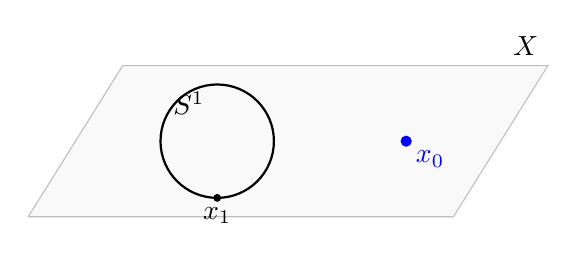
\begin{tikzpicture}[scale=1.2]
        % Plano X
        \draw[gray!50, fill=gray!5] (-2,-0.8) -- (2.5,-0.8) -- (3.5,0.8) -- (-1,0.8) -- cycle;
        \node[above left] at (3.5,0.8) {$X$};

        % Circulo S^1
        \draw[thick] (0,0) circle (0.6);
        \node at (-0.3, 0.4) {$S^1$};
        \filldraw (0,-0.6) circle (1pt) node[below] {$x_1$};

        % Punto aislado x_0
        \filldraw[blue] (2,0) circle (1.5pt) node[below right] {$x_0$};
    \end{tikzpicture}
    \caption{Spazio $X = S^1 \cup \{x_0\}$ con un punto isolato $x_0$.}
\end{figure}

Chiaramente, per il punto isolato $x_0$ si ha $\Lambda_{x_0} = \{c_{x_0}\}$, quindi:
\[
\Pi_1(X, x_0) = \{[c_{x_0}]\} = 0
\]
Invece, per qualsiasi punto $x_1 \in S^1$, si ha:
\[
\Pi_1(X, x_1) \neq 0
\]
poiché non tutti i cappi contenuti in $S^1$ sono omotopi al cammino costante $c_{x_1}$. Questo mostra che, in generale, il gruppo fondamentale dipende dalla scelta del punto base se lo spazio non è connesso per archi. (Il fatto che $\Pi_1(S^1) \neq 0$ sarà dimostrato rigorosamente pi\`u avanti, con Seifert--Van Kampen: $\Pi_1(S^1) \cong \mathbb{Z}$.)
\end{ejemplo}

\vspace{1.5em}

\begin{teo}
Siano $X$ uno spazio topologico e $x_0, x_1 \in X$. Se esiste un cammino $\alpha: I \to X$ con $\alpha(0) = x_0$ e $\alpha(1) = x_1$, allora l'applicazione:
\Func{\alpha_*}{\Pi_1(X, x_0)}{\Pi_1(X, x_1)}{[\sigma]}{[\alpha^{-1} * \sigma * \alpha]}
è un \textbf{isomorfismo di gruppi}.
\end{teo}

\begin{proof}
Dimostriamo le tre proprietà dell'applicazione $\alpha_*$:

\begin{figure}[H]
    \centering
    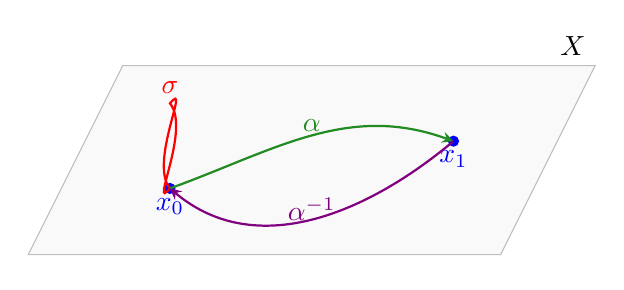
\begin{tikzpicture}[scale=1.2]
        % Plano X
        \draw[gray!50, fill=gray!5] (-2,-1) -- (3,-1) -- (4,1) -- (-1,1) -- cycle;
        \node[above left] at (4,1) {$X$};

        % Puntos x_0 y x_1
        \coordinate (X0) at (-0.5,-0.3);
        \coordinate (X1) at (2.5,0.2);
        \filldraw[blue] (X0) circle (1.5pt) node[below] {$x_0$};
        \filldraw[blue] (X1) circle (1.5pt) node[below] {$x_1$};

        % Lazo \sigma en x_0
        \draw[thick, red] (X0) to[out=130, in=50] (-0.5,0.6) to[out=-50, in=-130] (X0);
        \node[red, above] at (-0.5,0.6) {$\sigma$};

        % Cammino \alpha de x_0 a x_1
        \draw[thick, ForestGreen, ->, >=stealth] (X0) to[out=20, in=160] (2.5,0.2);
        \node[ForestGreen, above] at (1.0, 0.2) {$\alpha$};

        % Cammino \alpha^{-1}
        \draw[thick, Purple, ->, >=stealth] (X1) to[out=-140, in=-40] (X0);
        \node[Purple, below] at (1.0, -0.3) {$\alpha^{-1}$};
    \end{tikzpicture}
    \caption{Coniugazione di un cappio $\sigma$ in $x_0$ tramite il cammino $\alpha$.}
\end{figure}

\begin{itemize}
    \item \textbf{Buona definizione:} Per ogni $\sigma \in \Lambda_{x_0}$, la concatenazione $\alpha^{-1} * \sigma * \alpha$ è un cappio centrato in $x_1$, quindi $\alpha^{-1} * \sigma * \alpha \in \Lambda_{x_1}$.
    Inoltre, se $[\sigma] = [\sigma']$, ossia $\sigma \simeq \sigma' \text{ rel } \partial I$, allora poichè $\alpha \simeq \alpha \text{ rel } \partial I$ e $\alpha^{-1} \simeq \alpha^{-1} \text{ rel } \partial I$, si ha:
    \[
    \alpha^{-1} * \sigma * \alpha \simeq \alpha^{-1} * \sigma' * \alpha \text{ rel } \partial I \implies [\alpha^{-1} * \sigma * \alpha] = [\alpha^{-1} * \sigma' * \alpha]
    \]
    Quindi $\alpha_*$ non dipende dal rappresentante scelto.

    \item \textbf{Iniettività:} Siano $\sigma, \tau \in \Lambda_{x_0}$ tali che $\alpha_*([\sigma]) = \alpha_*([\tau])$.
    Allora $[\alpha^{-1} * \sigma * \alpha] = [\alpha^{-1} * \tau * \alpha]$, ossia $\alpha^{-1} * \sigma * \alpha \simeq \alpha^{-1} * \tau * \alpha \text{ rel } \partial I$.
    
    Concatenando a sinistra per $\alpha$ e a destra per $\alpha^{-1}$:
    \[
    \alpha * (\alpha^{-1} * \sigma * \alpha) * \alpha^{-1} \simeq \alpha * (\alpha^{-1} * \tau * \alpha) * \alpha^{-1} \text{ rel } \partial I
    \]
    Usando l'associatività e i risultati sugli elementi inversi e neutri ($\alpha * \alpha^{-1} \simeq c_{x_0}$):
    \[
    c_{x_0} * \sigma * c_{x_0} \simeq c_{x_0} * \tau * c_{x_0} \implies \sigma \simeq \tau \text{ rel } \partial I \implies [\sigma] = [\tau]
    \]
    Pertanto $\alpha_*$ è iniettiva.

    \item \textbf{Suriettività:} Sia $[\eta] \in \Pi_1(X, x_1)$ un qualsiasi elemento con $\eta \in \Lambda_{x_1}$.
    Poniamo $\sigma = \alpha * \eta * \alpha^{-1} \in \Lambda_{x_0}$. Calcolando l'immagine tramite $\alpha_*$:
    \[
    \alpha_*([\sigma]) = [\alpha^{-1} * (\alpha * \eta * \alpha^{-1}) * \alpha] = [(\alpha^{-1} * \alpha) * \eta * (\alpha^{-1} * \alpha)]
    \]
    Poiché $\alpha^{-1} * \alpha \simeq c_{x_1} \text{ rel } \partial I$, si ottiene:
    \[
    c_{x_1} * \eta * c_{x_1} \simeq \eta \text{ rel } \partial I \implies \alpha_*([\sigma]) = [\eta]
    \]
    Quindi $\alpha_*$ è suriettiva.

    \item \textbf{Omomorfismo di gruppi:} Siano $\sigma, \tau \in \Lambda_{x_0}$:
    \[
    \alpha_*([\sigma]) \cdot \alpha_*([\tau]) = [\alpha^{-1} * \sigma * \alpha] \cdot [\alpha^{-1} * \tau * \alpha] = [\alpha^{-1} * \sigma * (\alpha * \alpha^{-1}) * \tau * \alpha]
    \]
    Essendo $\alpha * \alpha^{-1} \simeq c_{x_0} \text{ rel } \partial I$:
    \[
    [\alpha^{-1} * \sigma * c_{x_0} * \tau * \alpha] = [\alpha^{-1} * (\sigma * \tau) * \alpha] = \alpha_*([\sigma * \tau]) = \alpha_*([\sigma] \cdot [\tau])
    \]
\end{itemize}
Dunque $\alpha_*$ è un isomorfismo di gruppi.
\end{proof}

\begin{coro}
Sia $X$ uno spazio topologico connesso per archi. Allora il gruppo fondamentale $\Pi_1(X, x)$ è isomorfo per tutti i punti $x \in X$ (ed è quindi indipendente dal punto base a meno di isomorfismo, potendo scriverlo semplicemente $\Pi_1(X)$).
\end{coro}

\begin{observacion}
Se $X$ è uno spazio topologico e $x_0 \in X$, la condizione $\Pi_1(X, x_0) = 0$ equivale a dire che ogni cappio in $x_0$ è omotopo al cammino costante $c_{x_0}$ relativamente al bordo $\partial I$. Ciò equivale a dire che per ogni coppia di cammini $\alpha, \beta: I \to X$ con $\alpha(0) = \beta(0) = x_0$ e $\alpha(1) = \beta(1)$, si ha $\alpha \simeq \beta \text{ rel } \partial I$.
\end{observacion}

\begin{proof}[Dimostrazione dell'equivalenza]
($\Leftarrow$) Basta applicare l'ipotesi con $\alpha = \sigma$ (un cappio in $x_0$) e $\beta = c_{x_0}$.

($\Rightarrow$) Siano $\alpha, \beta$ con $\alpha(0) = \beta(0) = x_0$ e $\alpha(1) = \beta(1) = x_1$. Allora $\alpha * \beta^{-1} \in \Lambda_{x_0}$, e poich\'e $\Pi_1(X, x_0) = 0$ si ha $\alpha * \beta^{-1} \simeq c_{x_0}$ rel $\partial I$. Usando compatibilit\`a, associativit\`a, inverso e neutro:
\[
\alpha \simeq \alpha * c_{x_1} \simeq \alpha * (\beta^{-1} * \beta) \simeq (\alpha * \beta^{-1}) * \beta \simeq c_{x_0} * \beta \simeq \beta \quad \text{rel } \partial I. \qedhere
\]
\end{proof}

\section{Invarianza Topologica del Gruppo Fondamentale}

\begin{prop}
Siano $X, Y$ spazi topologici, $x_0 \in X$ e $f: X \to Y$ un'applicazione continua.
Allora l'applicazione indotta da $f$:
\Func{f_*}{\Pi_1(X, x_0)}{\Pi_1(Y, f(x_0))}{[\sigma]}{[f \circ \sigma]}
è un \textbf{omomorfismo di gruppi} (più precisamente indicato con $f_{*x_0}$).
\end{prop}

\begin{proof}
Verifichiamo le due proprietà:
\begin{itemize}
    \item \textbf{Buona definizione:} Per ogni $\sigma \in \Lambda_{x_0}(X)$, la composizione $f \circ \sigma$ è un cappio in $Y$ centrato in $f(x_0)$, ossia $f \circ \sigma \in \Lambda_{f(x_0)}(Y)$.
    Se $[\sigma] = [\sigma']$, si ha $\sigma \simeq \sigma' \text{ rel } \partial I$. Sia $H: \sigma \simeq \sigma' \text{ rel } \partial I$. Allora $f \circ H: I \times I \to Y$ \`e continua, $(f\circ H)(t,0) = f(\sigma(t))$, $(f \circ H)(t,1) = f(\sigma'(t))$ e $(f \circ H)(0,s) = f(x_0) = (f\circ H)(1,s)$. Dunque $f \circ \sigma \simeq f \circ \sigma' \text{ rel } \partial I$ (\`e un caso particolare del teorema di compatibilit\`a con la composizione, con la omotopia costante $f \simeq f$), quindi $[f \circ \sigma] = [f \circ \sigma']$.

    \item \textbf{Omomorfismo:} Siano $\sigma, \tau \in \Lambda_{x_0}(X)$. Osserviamo che per ogni $t \in I$:
    \[
    (f \circ (\sigma * \tau))(t) = 
    \begin{cases}
        f(\sigma(2t)) & t \leqslant 1/2 \\
        f(\tau(2t-1)) & t \geqslant 1/2
    \end{cases}
    = ((f \circ \sigma) * (f \circ \tau))(t)
    \]
    Quindi $f \circ (\sigma * \tau) = (f \circ \sigma) * (f \circ \tau)$. Di conseguenza:
    \[
    f_*([\sigma] \cdot [\tau]) = f_*([\sigma * \tau]) = [f \circ (\sigma * \tau)] = [(f \circ \sigma) * (f \circ \tau)] = f_*([\sigma]) \cdot f_*([\tau])
    \]
\end{itemize}
\end{proof}

\vspace{1em}

\begin{prop}
\begin{enumerate}[label=\alph*)]
    \item Siano $X, Y, Z$ spazi topologici, $x_0 \in X$, $f: X \to Y$ e $g: Y \to Z$ continue. Allora:
    \[
    (g \circ f)_* = g_* \circ f_* \quad \text{su } \Pi_1(X, x_0)
    \]
    \item L'applicazione identità $\mathrm{Id}_X: X \to X$ induce l'identità sul gruppo fondamentale:
    \[
    (\mathrm{Id}_X)_* = \mathrm{Id}_{\Pi_1(X, x_0)}
    \]
\end{enumerate}
\end{prop}

\begin{proof}
\begin{itemize}
    \item[a)] Per ogni $[\sigma] \in \Pi_1(X, x_0)$:
    \[
    (g \circ f)_*([\sigma]) = [(g \circ f) \circ \sigma] = [g \circ (f \circ \sigma)] = g_*([f \circ \sigma]) = g_*(f_*([\sigma])) = (g_* \circ f_*)([\sigma])
    \]
    \item[b)] Per ogni $[\sigma] \in \Pi_1(X, x_0)$:
    \[
    (\mathrm{Id}_X)_*([\sigma]) = [\mathrm{Id}_X \circ \sigma] = [\sigma] = \mathrm{Id}_{\Pi_1(X, x_0)}([\sigma])
    \]
\end{itemize}
\end{proof}

\vspace{1.5em}

\begin{teo}[Invarianza Topologica]
Siano $X, Y$ spazi topologici, $x_0 \in X$ e $f: X \to Y$ un \textbf{omeomorfismo}. Poniamo $y_0 = f(x_0) \in Y$.
Allora l'applicazione indotta:
\[
f_*: \Pi_1(X, x_0) \longrightarrow \Pi_1(Y, y_0)
\]
è un \textbf{isomorfismo di gruppi}.
\end{teo}

\begin{proof}
Poiché $f$ è un omeomorfismo, esiste l'inversa continua $f^{-1}: Y \to X$ tale che $f^{-1} \circ f = \mathrm{Id}_X$ e $f \circ f^{-1} = \mathrm{Id}_Y$.
Applicando le proprietà di composizione per le mappe indotte:
\[
(f^{-1} \circ f)_* = (f^{-1})_* \circ f_* = (\mathrm{Id}_X)_* = \mathrm{Id}_{\Pi_1(X, x_0)}
\]
\[
(f \circ f^{-1})_* = f_* \circ (f^{-1})_* = (\mathrm{Id}_Y)_* = \mathrm{Id}_{\Pi_1(Y, y_0)}
\]
Quindi $f_*$ è un omomorfismo invertibile, la cui inversa è $(f_*)^{-1} = (f^{-1})_*$. Pertanto $f_*$ è un isomorfismo di gruppi\hfill$\square$
\end{proof}

\begin{coro}
Siano $X, Y$ spazi topologici connessi per archi. Se $X \cong Y$ (sono omeomorfi), allora $\Pi_1(X) \cong \Pi_1(Y)$.
\end{coro}

\begin{observacion}
Il viceversa non vale in generale. Ad esempio, consideriamo $X = \mathbb{R}^n$ e $Y = \{y_0\}$. Chiaramente $\mathbb{R}^n \not\cong \{y_0\}$ per $n \geqslant 1$. Tuttavia, $\Pi_1(\mathbb{R}^n) \cong \Pi_1(\{y_0\}) = 0$.
\end{observacion}

\vspace{2em}

\section{Invarianza Omotopica del Gruppo Fondamentale}

\begin{lema}
Siano $X, Y$ spazi topologici e $f_1, f_2: X \to Y$ mappe continue tali che $H: f_1 \simeq f_2$ (con $H: X \times I \to Y$ l'omotopia).
Fissato $x_0 \in X$, sia $\alpha: I \to Y$ il cammino in $Y$ definito da $\alpha(s) = H(x_0, s)$, che connette $f_1(x_0)$ ad $f_2(x_0)$ (ossia $\alpha(0) = f_1(x_0)$ e $\alpha(1) = f_2(x_0)$).

Allora vale la seguente relazione tra gli omomorfismi indotti:
\[
\alpha_* \circ (f_1)_* = (f_2)_*
\]

\begin{figure}[H]
    \centering
    \begin{tikzcd}[scale=1.3]
        \Pi_1(X, x_0) \arrow[r, "(f_1)_*"] \arrow[dr, "(f_2)_*"'] & \Pi_1(Y, f_1(x_0)) \arrow[d, "\alpha_*"] \\
        & \Pi_1(Y, f_2(x_0))
    \end{tikzcd}
    \caption{Diagramma commutativo per l'omomorfismo indotto tra mappe omotope.}
\end{figure}
\end{lema}

\begin{proof}[Dimostrazione (Facoltativa)]
Dobbiamo dimostrare che per ogni $\sigma \in \Lambda_{x_0}(X)$ si ha $(f_2)_*([\sigma]) = (\alpha_* \circ (f_1)_*)([\sigma])$, ossia $[f_2 \circ \sigma] = [\alpha^{-1} * (f_1 \circ \sigma) * \alpha]$\hfill(*)

Sia $H: X \times I \to Y$ l'omotopia tra $f_1$ e $f_2$.
Notiamo che il cammino coniugato si scrive come:
\[
(\alpha^{-1} * (f_1 \circ \sigma) * \alpha)(t) = 
\begin{cases}
    \alpha^{-1}(4t) = \alpha(1-4t) = H(x_0, 1-4t) & t \leqslant 1/4 \\
    (f_1 \circ \sigma)(4t-1) = H(\sigma(4t-1), 0) & 1/4 \leqslant t \leqslant 1/2 \\
    \alpha(2t-1) = H(x_0, 2t-1) & t \geqslant 1/2
\end{cases}
\]

D'altra parte, il cammino $f_2 \circ \sigma$ verifica $f_2(\sigma(t)) = H(\sigma(t), 1)$ per ogni $t \in I$. Ponendo $y_0 = f_2(x_0)$, si ha anche la decomposizione con cappi costanti:
\[
f_2 \circ \sigma \simeq (c_{y_0} * (f_2 \circ \sigma)) * c_{y_0} \text{ rel } \partial I
\]
dove
\[
(c_{y_0} * (f_2 \circ \sigma) * c_{y_0})(t) = 
\begin{cases}
    y_0 = f_2(x_0) = H(x_0, 1) & t \leqslant 1/4 \\
    H(\sigma(4t-1), 1) & 1/4 \leqslant t \leqslant 1/2 \\
    H(x_0, 1) & t \geqslant 1/2
\end{cases}
\]

Definiamo ora la mappa di omotopia $K: I \times I \to Y$:
\[
K(t,s) = 
\begin{cases}
    H(x_0, 1 - 4t(1-s)) & t \leqslant 1/4 \\[0.5em]
    H(\sigma(4t-1), s) & 1/4 \leqslant t \leqslant 1/2 \\[0.5em]
    H(x_0, 1 - 2(1-t)(1-s)) & t \geqslant 1/2
\end{cases}
\]

Controlliamo la continuità sulle giunzioni $t = 1/4$ e $t = 1/2$:
\begin{itemize}
    \item Per $t = 1/4$: $H(x_0, 1 - 1(1-s)) = H(x_0, s) = H(\sigma(0), s)$.
    \item Per $t = 1/2$: $H(\sigma(1), s) = H(x_0, s) = H(x_0, 1 - 2(1/2)(1-s)) = H(x_0, s)$.
\end{itemize}
Per il Lemma di Incollamento, $K$ è ben definita e continua.

Verifichiamo le condizioni ai bordi per la variabile $s$:
\begin{enumerate}[label=\roman*)]
    \item Per $s = 0$: $K(t,0) = (\alpha^{-1} * (f_1 \circ \sigma) * \alpha)(t)$.
    \item Per $s = 1$: $K(t,1) = (c_{y_0} * (f_2 \circ \sigma) * c_{y_0})(t)$.
    \item Per ogni $s \in I$: $K(0,s) = H(x_0, 1) = f_2(x_0) = y_0$ e $K(1,s) = H(x_0, 1) = y_0$.
\end{enumerate}
Pertanto $K: \alpha^{-1} * (f_1 \circ \sigma) * \alpha \simeq c_{y_0} * (f_2 \circ \sigma) * c_{y_0} \text{ rel } \partial I$. Poich\'e, per la propriet\`a dell'elemento neutro, $c_{y_0} * (f_2 \circ \sigma) * c_{y_0} \simeq f_2 \circ \sigma \text{ rel } \partial I$, per transitivit\`a si ottiene $\alpha^{-1} * (f_1 \circ \sigma) * \alpha \simeq f_2 \circ \sigma \text{ rel } \partial I$, cio\`e (*), ossia $\alpha_* \circ (f_1)_* = (f_2)_*$\hfill$\square$
\end{proof}

\vspace{1.5em}

\begin{teo}[Invarianza Omotopica del Gruppo Fondamentale]
Siano $X, Y$ spazi topologici omotopicamente equivalenti ($X \simeq Y$), e siano $f: X \to Y$ e $g: Y \to X$ mappe continue tali che $g \circ f \simeq \mathrm{Id}_X$ e $f \circ g \simeq \mathrm{Id}_Y$.
Allora per ogni $x_0 \in X$, l'applicazione indotta:
\[
f_*: \Pi_1(X, x_0) \longrightarrow \Pi_1(Y, f(x_0))
\]
è un \textbf{isomorfismo di gruppi}.
\end{teo}

\begin{proof}
\textbf{Passo 1: $f_*$ \`e iniettiva (e $g_*$ \`e suriettiva).} Sia $H: \mathrm{Id}_X \simeq g \circ f$ e sia $\alpha(s) = H(x_0, s)$, cammino da $x_0$ a $(g \circ f)(x_0)$. Applicando il Lemma a $f_1 = \mathrm{Id}_X$ e $f_2 = g \circ f$ si ottiene il diagramma commutativo

\begin{center}
\begin{tikzcd}
\Pi_1(X, x_0) \arrow[r, "(\mathrm{Id}_X)_*"] \arrow[dr, "(g \circ f)_*"'] & \Pi_1(X, x_0) \arrow[d, "\alpha_*"] \\
 & \Pi_1(X, (g \circ f)(x_0))
\end{tikzcd}
\end{center}

cio\`e $(g \circ f)_* = \alpha_* \circ (\mathrm{Id}_X)_* = \alpha_*$, che \`e un isomorfismo (Teorema del cambio di punto base). Poich\'e $(g \circ f)_* = g_* \circ f_*$, ne segue che $f_*: \Pi_1(X, x_0) \to \Pi_1(Y, f(x_0))$ \`e \textbf{iniettiva} e che $g_*: \Pi_1(Y, f(x_0)) \to \Pi_1(X, (g\circ f)(x_0))$ \`e \textbf{suriettiva}.

\textbf{Passo 2: $g_*$ \`e iniettiva.} Il ruolo di $f$ e $g$ \`e simmetrico: da $f \circ g \simeq \mathrm{Id}_Y$ e dal Passo 1 (applicato a $g$, con punto base $y_1 = f(x_0)$ e omotopia $K: \mathrm{Id}_Y \simeq f \circ g$) segue che $g_*: \Pi_1(Y, y_1) \to \Pi_1(X, g(y_1))$ \`e iniettiva.

\textbf{Passo 3: conclusione.} Per i Passi 1 e 2, $g_*: \Pi_1(Y, f(x_0)) \to \Pi_1(X, (g\circ f)(x_0))$ \`e un isomorfismo. Da $g_* \circ f_* = \alpha_*$ si ricava
\[
f_* = (g_*)^{-1} \circ \alpha_* ,
\]
composizione di due isomorfismi: dunque $f_*$ \`e un isomorfismo di gruppi\hfill$\square$
\end{proof}

\begin{observacion}[Sull'enunciato negli appunti]
Negli appunti il teorema \`e enunciato per ogni $x_0 \in g(Y)$, e la dimostrazione usa un $y_0 \in Y$ con $g(y_0) = x_0$: \emph{per quell'ipotesi l'argomento degli appunti \`e corretto}. Infatti, per $x_0 = g(y_0)$, sia $K: \mathrm{Id}_Y \simeq f \circ g$ e $\beta(s) = K(y_0, s)$ (da $y_0$ a $f(g(y_0)) = f(x_0)$): per il Lemma, $f_{*x_0} \circ g_{*y_0} = (f \circ g)_* = \beta_* \circ (\mathrm{Id}_Y)_* = \beta_*$ \`e un isomorfismo, quindi $f_{*x_0}$ \`e suriettiva (ed \`e iniettiva per il Passo 1). (Nella trascrizione automatica l'ipotesi $x_0 \in g(Y)$ si era persa, e nella precedente revisione l'argomento era stato giudicato erroneo per questo motivo: la valutazione era ingiusta.) La dimostrazione data qui sopra, invece, prova l'enunciato pi\`u forte, valido per \emph{ogni} $x_0 \in X$, anche fuori da $g(Y)$.
\end{observacion}

\begin{coro}
Siano $X, Y$ spazi topologici connessi per archi. Se $X \simeq Y$ (sono omotopicamente equivalenti), allora $\Pi_1(X) \cong \Pi_1(Y)$.
\end{coro}

\begin{observacion}
Il viceversa non è vero in generale. Ad esempio, prendendo $X = S^2$ e $Y = \{y_0\}$, si ha $\Pi_1(S^2) = 0 = \Pi_1(\{y_0\})$, ma $S^2 \not\simeq \{y_0\}$ in quanto $S^2$ non è uno spazio contraibile ($\mathrm{Id}_{S^2} \not\simeq -\mathrm{Id}_{S^2}$).
\end{observacion}

\vspace{1.5em}

\begin{ejemplo}[Calcolo dei Gruppi Fondamentali per Spazi Notevoli]
\begin{enumerate}
    \item Per ogni spazio topologico contraibile $X$, si ha $\Pi_1(X) = 0$.
    Infatti, $X \simeq \{y_0\} \implies \Pi_1(X) \cong \Pi_1(\{y_0\}) = 0$.
    Esempi tipici: $\mathbb{R}^n$, insiemi convessi $\Omega \subseteq \mathbb{R}^n$ e insiemi stellati $S \subseteq \mathbb{R}^n$.

    \item Per lo spazio euclideo bucato nell'origine:
    \[
    \Pi_1(\mathbb{R}^n \setminus \{\bar{0}\}) \cong \Pi_1(S^{n-1})
    \]
    poiché $S^{n-1}$ è un retratto di deformazione di $\mathbb{R}^n \setminus \{\bar{0}\}$.

    \item Per la sfera privata di due punti distinti $p \neq q$:
    \[
    \Pi_1(S^n \setminus \{p,q\}) \cong \Pi_1(S^{n-1})
    \]
    in quanto $S^n \setminus \{p,q\} \cong S^n \setminus \{N, S\} \simeq S^{n-1}$.
\end{enumerate}
\end{ejemplo}

\section{Il Gruppo Fondamentale dello Spazio Prodotto}

\begin{teo}
Siano $X, Y$ spazi topologici, $x_0 \in X$ e $y_0 \in Y$.
Allora il gruppo fondamentale del prodotto cartesiano $X \times Y$ è isomorfo al prodotto diretto dei gruppi fondamentali:
\[
\Pi_1(X \times Y, (x_0, y_0)) \cong \Pi_1(X, x_0) \times \Pi_1(Y, y_0)
\]
\end{teo}

\begin{proof}
Siano $p_1: X \times Y \to X$ e $p_2: X \times Y \to Y$ le proiezioni canoniche definite da $p_1(x,y) = x$ e $p_2(x,y) = y$.
Essendo $p_1$ e $p_2$ continue, esse inducono gli omomorfismi di gruppi $p_{1*}: \Pi_1(X \times Y, (x_0, y_0)) \to \Pi_1(X, x_0)$ e $p_{2*}: \Pi_1(X \times Y, (x_0, y_0)) \to \Pi_1(Y, y_0)$.

Definiamo l'applicazione:
\Func{\Phi}{\Pi_1(X \times Y, (x_0, y_0))}{\Pi_1(X, x_0) \times \Pi_1(Y, y_0)}{[\eta]}{(p_{1*}([\eta]), \, p_{2*}([\eta])) = ([p_1 \circ \eta], \, [p_2 \circ \eta])}

Verifichiamo che $\Phi$ sia un isomorfismo di gruppi:

\begin{itemize}
    \item \textbf{$\Phi$ è un omomorfismo:} Per ogni $[\eta], [\eta'] \in \Pi_1(X \times Y, (x_0, y_0))$:
    \[
    \begin{aligned}
        \Phi([\eta] \cdot [\eta']) &= (p_{1*}([\eta] \cdot [\eta']), \, p_{2*}([\eta] \cdot [\eta'])) \\
        &= (p_{1*}([\eta]) \cdot p_{1*}([\eta']), \, p_{2*}([\eta]) \cdot p_{2*}([\eta'])) \\
        &= (p_{1*}([\eta]), \, p_{2*}([\eta])) \cdot (p_{1*}([\eta']), \, p_{2*}([\eta'])) = \Phi([\eta]) \cdot \Phi([\eta'])
    \end{aligned}
    \]

    \item \textbf{$\Phi$ è suriettiva:} Siano $\sigma \in \Lambda_{x_0}(X)$ e $\tau \in \Lambda_{y_0}(Y)$.
    Definiamo il cappio $\eta: I \to X \times Y$ tramite $\eta(t) = (\sigma(t), \tau(t))$. Poiché le sue componenti sono continue, $\eta$ è continua e $\eta \in \Lambda_{(x_0, y_0)}(X \times Y)$.
    Calcolando l'immagine:
    \[
    \Phi([\eta]) = ([p_1 \circ \eta], [p_2 \circ \eta]) = ([\sigma], [\tau])
    \]
    Quindi $\Phi$ è suriettiva.

    \item \textbf{$\Phi$ è iniettiva:} Siano $\eta, \eta' \in \Lambda_{(x_0, y_0)}(X \times Y)$ tali che $\Phi([\eta]) = \Phi([\eta'])$.
    Allora $(p_{1*}([\eta]), p_{2*}([\eta])) = (p_{1*}([\eta']), p_{2*}([\eta'])) \implies [p_1 \circ \eta] = [p_1 \circ \eta']$ e $[p_2 \circ \eta] = [p_2 \circ \eta']$.
    
    Quindi esistono due omotopie relative al bordo:
    \[
    H: p_1 \circ \eta \simeq p_1 \circ \eta' \text{ rel } \partial I \quad \text{e} \quad K: p_2 \circ \eta \simeq p_2 \circ \eta' \text{ rel } \partial I
    \]
    Poniamo l'omotopia prodotto $W: I \times I \to X \times Y$ definita da $W(t,s) = (H(t,s), K(t,s))$.
    $W$ è continua e soddisfa:
    \begin{enumerate}[label=\roman*)]
        \item $W(t,0) = (H(t,0), K(t,0)) = ((p_1 \circ \eta)(t), (p_2 \circ \eta)(t)) = \eta(t)$.
        \item $W(t,1) = (H(t,1), K(t,1)) = ((p_1 \circ \eta')(t), (p_2 \circ \eta')(t)) = \eta'(t)$.
        \item $W(0,s) = (x_0, y_0) = W(1,s)$ per ogni $s \in I$.
    \end{enumerate}
    Pertanto $W: \eta \simeq \eta' \text{ rel } \partial I \implies [\eta] = [\eta']$, dimostrando l'iniettività.
\end{itemize}
In conclusione, $\Phi$ è un isomorfismo di gruppi\hfill$\square$
\end{proof}

\vspace{1.5em}

\begin{ejemplo}
Calcolo del gruppo fondamentale per prodotti topologici notevoli:

\begin{enumerate}
    \item \textbf{Cilindro vuoto:} $X = S^1 \times I$ oppure $S^1 \times \mathbb{R}$.
    \[
    \Pi_1(S^1 \times I) \cong \Pi_1(S^1) \times \Pi_1(I) \cong \mathbb{Z} \times \{0\} \cong \mathbb{Z}
    \]
    Geometricamente, $\mathbb{Z}$ conta il numero di avvolgimenti (con segno) che un cappio compie attorno a $S^1$.

    \item \textbf{Toro bidimensionale (Superficie torica):} $X = T^2 = S^1 \times S^1$.
    \[
    \Pi_1(T^2) = \Pi_1(S^1 \times S^1) \cong \Pi_1(S^1) \times \Pi_1(S^1) \cong \mathbb{Z} \times \mathbb{Z} = \mathbb{Z}^2
    \]

    \item \textbf{Toro pieno:} $X = S^1 \times B^2$.
    Poiché il disco chiuso $B^2$ è convesso (e quindi contraibile, $\Pi_1(B^2) = 0$):
    \[
    \Pi_1(S^1 \times B^2) \cong \Pi_1(S^1) \times \Pi_1(B^2) \cong \mathbb{Z} \times \{0\} \cong \mathbb{Z}
    \]
\end{enumerate}

\begin{figure}[H]
    \centering
    \begin{subfigure}[b]{0.3\textwidth}
        \centering
        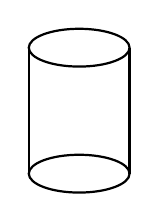
\begin{tikzpicture}[scale=0.8]
            \draw[thick] (0,0) ellipse (0.8cm and 0.3cm);
            \draw[thick] (0,2) ellipse (0.8cm and 0.3cm);
            \draw[thick] (-0.8,0) -- (-0.8,2);
            \draw[thick] (0.8,0) -- (0.8,2);
        \end{tikzpicture}
        \caption{Cilindro $S^1 \times I$}
    \end{subfigure}
    \hfill
    \begin{subfigure}[b]{0.3\textwidth}
        \centering
        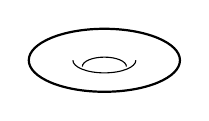
\begin{tikzpicture}[scale=0.8]
            \draw[thick] (0,0) ellipse (1.2cm and 0.5cm);
            \draw (-0.5,0) arc (180:360:0.5cm and 0.2cm);
            \draw (-0.35,-0.1) arc (180:0:0.35cm and 0.15cm);
        \end{tikzpicture}
        \caption{Toro $T^2 = S^1 \times S^1$}
    \end{subfigure}
    \hfill
    \begin{subfigure}[b]{0.3\textwidth}
        \centering
        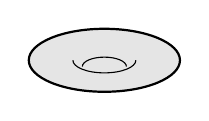
\begin{tikzpicture}[scale=0.8]
            \draw[thick, fill=gray!20] (0,0) ellipse (1.2cm and 0.5cm);
            \draw (-0.5,0) arc (180:360:0.5cm and 0.2cm);
            \draw (-0.35,-0.1) arc (180:0:0.35cm and 0.15cm);
        \end{tikzpicture}
        \caption{Toro pieno $S^1 \times B^2$}
    \end{subfigure}
    \caption{Rappresentazione grafica degli spazi prodotto.}
\end{figure}
\end{ejemplo}

\vspace{2em}

\section{Il Toro $n$-Dimensionale}

\begin{definicion}[\textbf{IMPORTANTE PER L'ESAME}]
Si chiama \textbf{toro $n$-dimensionale} lo spazio topologico quoziente:
\[
T^n = \mathbb{R}^n \big/ \mathbb{Z}^n
\]
dotato della topologia quoziente indotta dalla topologia naturale su $\mathbb{R}^n$.

Un ruolo fondamentale è svolto dalla \textbf{proiezione canonica suriettiva}:
\Func{\pi}{\mathbb{R}^n}{T^n = \mathbb{R}^n / \mathbb{Z}^n}{x}{[x]_{\mathbb{Z}^n} = x + \mathbb{Z}^n}

Per ogni $x, y \in \mathbb{R}^n$, la relazione di equivalenza è data da:
\[
x \sim_\pi y \iff \pi(x) = \pi(y) \iff x - y \in \mathbb{Z}^n \iff x_i - y_i \in \mathbb{Z}, \quad \forall i = 1, \dots, n
\]
\end{definicion}

\begin{prop}
Sia $Q = I^n = [0,1]^n$ il cubo unitario $n$-dimensionale.
La restrizione della proiezione canonica $\pi|_Q: Q \to T^n$ è continua e suriettiva, e identifica $T^n \cong Q / \sim$.
\end{prop}

\begin{proof}
Dimostriamo che $\pi(Q) = T^n$:
\begin{itemize}
    \item [$\subseteq$)] Banale poiché $Q \subset \mathbb{R}^n \implies \pi(Q) \subseteq \pi(\mathbb{R}^n) = T^n$.
    \item [$\supseteq$)] Sia $y = (y_1, \dots, y_n) \in \mathbb{R}^n$. Per ogni $i = 1, \dots, n$, definiamo $x_i = y_i - \lfloor y_i \rfloor$, dove $\lfloor y_i \rfloor$ indica la parte intera.
    Allora $x_i \in [0,1]$ per ogni $i$, il che implica $x = (x_1, \dots, x_n) \in Q = I^n$.
    Inoltre $y - x = (\lfloor y_1 \rfloor, \dots, \lfloor y_n \rfloor) \in \mathbb{Z}^n$, quindi $\pi(x) = \pi(y)$.
\end{itemize}
Pertanto $\pi(Q) = T^n$, ovvero la mappa è suriettiva.

\textbf{Identificazione $T^n \cong Q/\!\sim$.} Su $Q$ la relazione indotta da $\pi$ \`e $x \sim y \iff x - y \in \mathbb{Z}^n$: poich\'e $x,y \in [0,1]^n$, ci\`o accade solo se $x = y$ oppure se $x,y$ stanno su facce opposte del cubo con le restanti coordinate uguali (ad esempio, per $n=2$: $(0,y) \sim (1,y)$ e $(x,0) \sim (x,1)$). Inoltre $\pi|_Q$ \`e una applicazione continua e suriettiva da uno spazio compatto ($Q$) a uno spazio di Hausdorff ($T^n \cong S^1 \times \dots \times S^1$, vedi il teorema seguente); dunque \`e chiusa, e quindi una applicazione quoziente. Ne segue che $\pi|_Q$ induce un omeomorfismo $Q/\!\sim\ \cong T^n$\hfill$\square$
\end{proof}

\begin{coro}
Il toro $n$-dimensionale $T^n$ è uno spazio topologico \textbf{compatto}.
Infatti, $T^n = \pi(Q)$ è l'immagine continua di $Q = [0,1]^n$, che è compatto in $\mathbb{R}^n$ per il Teorema di Heine-Borel.
\end{coro}

\vspace{1.5em}

\begin{teo}
Il toro $n$-dimensionale è omeomorfo al prodotto cartesiano di $n$ circonferenze:
\[
T^n \cong \underbrace{S^1 \times \dots \times S^1}_{n \text{ volte}}
\]
\end{teo}

\begin{proof}
Analizziamo prima il caso $n = 1$:
Consideriamo la mappa esponenziale $p: \mathbb{R} \to S^1$ data da $p(t) = e^{2\pi i t} = (\cos(2\pi t), \sin(2\pi t))$.
$p$ è continua, suriettiva e aperta (\`e aperta perch\'e l'immagine di un intervallo aperto di lunghezza $\leqslant 1$ \`e un arco aperto di $S^1$, e ogni aperto di $\mathbb{R}$ \`e unione di tali intervalli).
Due punti $t, t' \in \mathbb{R}$ soddisfano $p(t) = p(t') \iff e^{2\pi i t} = e^{2\pi i t'} \iff t - t' \in \mathbb{Z}$.
Per il Teorema Fondamentale dell'Omeomorfismo Quoziente, $p$ induce un omeomorfismo $\tilde{p}: \mathbb{R}/\mathbb{Z} \xrightarrow{\cong} S^1$.

In generale per $n \geqslant 1$, definiamo la mappa:
\Func{\Phi}{\mathbb{R}^n}{\underbrace{S^1 \times \dots \times S^1}_{n \text{ volte}}}{(x_1, \dots, x_n)}{(p(x_1), \dots, p(x_n))}
$\Phi$ è ben posta, continua, suriettiva e aperta.
Inoltre, $\Phi(x) = \Phi(y) \iff x - y \in \mathbb{Z}^n$.
Pertanto, $\Phi$ induce un omeomorfismo sul quoziente:
\[
\widetilde{\Phi}: \mathbb{R}^n / \mathbb{Z}^n \xrightarrow{\;\cong\;} S^1 \times \dots \times S^1
\]
\end{proof}

\begin{coro}
Il gruppo fondamentale del toro $n$-dimensionale è:
\[
\Pi_1(T^n) \cong \Pi_1(S^1 \times \dots \times S^1) \cong \underbrace{\mathbb{Z} \times \dots \times \mathbb{Z}}_{n \text{ volte}} = \mathbb{Z}^n
\]
\end{coro}

\begin{figure}[H]
    \centering
    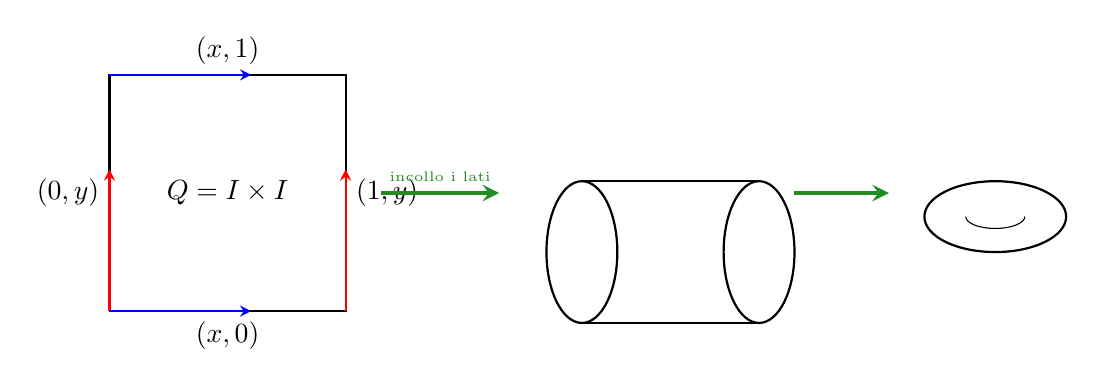
\begin{tikzpicture}[scale=1.5]
        % Cuadrado Q
        \draw[thick] (0,0) -- (2,0) node[midway, below] {$(x,0)$} -- (2,2) node[midway, right] {$(1,y)$} -- (0,2) node[midway, above] {$(x,1)$} -- (0,0) node[midway, left] {$(0,y)$};
        
        % Flechas de identificación
        \draw[thick, red, ->, >=stealth] (0,0) -- (0,1.2);
        \draw[thick, red, ->, >=stealth] (2,0) -- (2,1.2);
        \draw[thick, blue, ->, >=stealth] (0,0) -- (1.2,0);
        \draw[thick, blue, ->, >=stealth] (0,2) -- (1.2,2);

        \node at (1,1) {$Q = I \times I$};

        % Proceso de enrollado
        \draw[->, >=stealth, ForestGreen, ultra thick] (2.3, 1) -- (3.3, 1) node[midway, above] {\tiny incollo i lati};

        % Cilindro intermedio
        \draw[thick] (4,0.5) ellipse (0.3cm and 0.6cm);
        \draw[thick] (5.5,0.5) ellipse (0.3cm and 0.6cm);
        \draw[thick] (4,1.1) -- (5.5,1.1);
        \draw[thick] (4,-0.1) -- (5.5,-0.1);

        \draw[->, >=stealth, ForestGreen, ultra thick] (5.8, 1) -- (6.6, 1);

        % Toro
        \draw[thick] (7.5,0.8) ellipse (0.6cm and 0.3cm);
        \draw (7.25,0.8) arc (180:360:0.25cm and 0.1cm);
    \end{tikzpicture}
    \caption{Costruzione del toro $T^2$ identificando i lati opposti del quadrato $Q = I \times I$.}
\end{figure}

\begin{ejercicio*}[\textbf{DOMANDA D'ESAME}]
\textbf{Quali sono i modelli topologici del toro $T^n$?}
\begin{enumerate}
    \item Il quoziente dello spazio euclideo: $\mathbb{R}^n / \mathbb{Z}^n$.
    \item Il prodotto cartesiano di circonferenze: $S^1 \times \dots \times S^1$.
    \item Il quoziente del cubo unitario con le facce opposte identificate: $Q/\!\sim\ = I^n/\!\sim$.
\end{enumerate}
\end{ejercicio*}

\section{Spazi Semplicemente Connessi}

\begin{definicion}
Uno spazio topologico $X$ si dice \textbf{semplicemente connesso} se:
\begin{enumerate}
    \item $X$ è connesso per archi, e
    \item $\Pi_1(X) = 0$ (ossia ha gruppo fondamentale banale).
\end{enumerate}
\end{definicion}

\begin{observacion}
La condizione $\Pi_1(X, x_0) = 0$ equivale a dire che per ogni coppia di cammini $\alpha, \beta: I \to X$ con $\alpha(0) = \beta(0) = x_0$ e $\alpha(1) = \beta(1)$, si ha $\alpha \simeq \beta \text{ rel } \partial I$.
\end{observacion}

\begin{prop}
Se $X$ è uno spazio topologico contraibile, allora $X$ è semplicemente connesso.
\end{prop}

\begin{proof}
Se $X$ è contraibile, allora $X$ è connesso per archi. Inoltre $X \simeq \{x_0\}$, per cui $\Pi_1(X) \cong \Pi_1(\{x_0\}) = 0$. Pertanto $X$ è semplicemente connesso.
\end{proof}

\begin{observacion}
Il viceversa della proposizione precedente \textbf{non} vale: semplicemente connesso $\centernot\implies$ contraibile.

Come controesempio, si consideri la sfera 2-dimensionale $S^2$. Si ha che $S^2$ è semplicemente connessa ($\Pi_1(S^2) = 0$), ma $S^2$ non è contraibile in quanto $\mathrm{Id}_{S^2} \not\simeq -\mathrm{Id}_{S^2}$.
\end{observacion}

\vspace{1.5em}


\vspace{1.5em}

\begin{lema}[Numero di Lebesgue, per l'intervallo]
Sia $\{A, B\}$ un ricoprimento aperto di $I = [0,1]$. Allora esiste $\delta > 0$ tale che ogni sottoinsieme di $I$ di diametro $< \delta$ \`e contenuto in $A$ oppure in $B$. In particolare esiste una suddivisione $0 = t_0 < t_1 < \dots < t_k = 1$ tale che ciascun intervallo $[t_{r-1}, t_r]$ \`e contenuto in $A$ oppure in $B$.
\end{lema}

\begin{proof}
Se $A = I$ o $B = I$ non c'\`e nulla da dimostrare. Altrimenti la funzione $\ell(t) = \max\{ d(t, I \setminus A),\, d(t, I \setminus B) \}$ \`e continua su $I$ e strettamente positiva (se $t \in A$, che \`e aperto, allora $d(t, I\setminus A) > 0$; analogamente per $B$). Per compattezza ha minimo $\delta > 0$. Se $\mathrm{diam}(T) < \delta$ e $t \in T$, supponiamo ad esempio $\ell(t) = d(t, I \setminus A) \geqslant \delta$: allora $T \subseteq \{u : |u - t| < \delta\} \subseteq A$. La suddivisione si ottiene prendendo $k$ con $1/k < \delta$ e $t_r = r/k$.
\end{proof}

\begin{teo}
La sfera $S^n$ è semplicemente connessa se e solo se $n \geqslant 2$.
\end{teo}

\begin{proof}
\begin{itemize}
    \item[$\implies$)] Mostriamo che per $n = 0, 1$ la sfera non \`e semplicemente connessa:
    \begin{itemize}
        \item Per $n = 0$: $S^0 = \{-1, 1\}$ non è connessa per archi.
        \item Per $n = 1$: $\Pi_1(S^1) \cong \mathbb{Z} \neq 0$ (dimostrato pi\`u avanti con Seifert--Van Kampen).
    \end{itemize}

    \item[$\impliedby$)] Sia $n \geqslant 2$.

    \textbf{Connessione per archi.} Per $x, y \in S^n$ con $y \neq -x$ il segmento $\overline{xy}$ non passa per l'origine, quindi $t \mapsto \frac{(1-t)x + ty}{\|(1-t)x + ty\|}$ \`e un cammino in $S^n$ da $x$ a $y$. Se $y = -x$ si sceglie $z \in S^n \setminus \{x, -x\}$ (esiste perch\'e $n \geqslant 2$) e si concatenano un cammino da $x$ a $z$ e uno da $z$ a $-x$.

    \textbf{Setup.} Siano $p \neq q$ in $S^n$, $U = S^n \setminus \{p\}$, $V = S^n \setminus \{q\}$. Sono aperti, $U \cong V \cong \mathbb{R}^n$ (proiezione stereografica), quindi contraibili e con $\Pi_1 = 0$. Inoltre $W = U \cap V = S^n \setminus \{p,q\} \cong \mathbb{R}^n \setminus \{\bar 0\}$ \`e connesso per archi perch\'e $n \geqslant 2$. Fissiamo $x_0 \in W$ e un cappio $\sigma$ in $x_0$: dobbiamo mostrare che $\sigma \simeq c_{x_0}$ rel $\partial I$.

    \textbf{Suddivisione.} $A = \sigma^{-1}(U)$ e $B = \sigma^{-1}(V)$ sono un ricoprimento aperto di $I$. Per il Lemma di Lebesgue esiste una suddivisione di $I$ in intervalli ciascuno inviato da $\sigma$ in $U$ oppure in $V$. Raggruppando intervalli consecutivi inviati nello stesso aperto, otteniamo $0 = t_0 < t_1 < \dots < t_h = 1$ con $\delta_j = [t_{j-1}, t_j]$ tali che $\sigma(\delta_j)$ sta in $U$ e $\sigma(\delta_{j+1})$ in $V$ o viceversa (alternati). Posto $x_j = \sigma(t_j)$, per $1 \leqslant j \leqslant h-1$ si ha
    \[
    x_j \in \sigma(\delta_j) \cap \sigma(\delta_{j+1}) \subseteq U \cap V = W .
    \]

    \textbf{Cammini di collegamento.} Poich\'e $W$ \`e connesso per archi, per $1 \leqslant j \leqslant h-1$ esiste $\tau_j: I \to W$ con $\tau_j(0) = x_0$, $\tau_j(1) = x_j$. Poniamo $\tau_0 = \tau_h = c_{x_0}$ (si ha $x_0 = \sigma(0) = \sigma(1)$).

    \begin{center}
    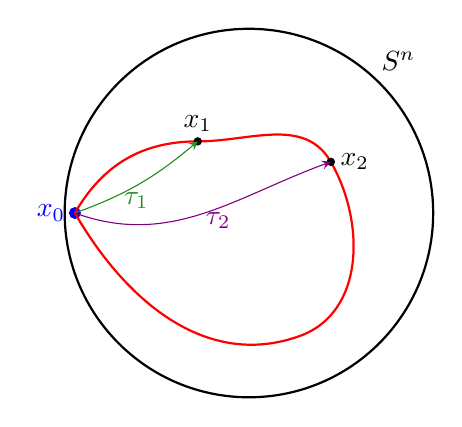
\begin{tikzpicture}[scale=1.3]
        \draw[thick] (0,0) circle (1.8cm);
        \node[above right] at (1.2,1.3) {$S^n$};
        \filldraw[blue] (-1.7, 0) circle (1.5pt) node[left] {$x_0$};
        \draw[thick, red] (-1.7,0) to[out=60, in=180] (-0.5,0.7) to[out=0, in=120] (0.8,0.5) to[out=-60, in=20] (0.5,-1.2) to[out=200, in=-60] (-1.7,0);
        \filldraw (-0.5,0.7) circle (1pt) node[above] {$x_1$};
        \filldraw (0.8,0.5) circle (1pt) node[right] {$x_2$};
        \draw[ForestGreen, ->, >=stealth] (-1.7,0) to[out=20, in=220] (-0.5,0.7);
        \node[ForestGreen, below] at (-1.1,0.3) {$\tau_1$};
        \draw[Purple, ->, >=stealth] (-1.7,0) to[out=-20, in=200] (0.8,0.5);
        \node[Purple, below] at (-0.3, 0.1) {$\tau_2$};
    \end{tikzpicture}
    \end{center}

    \textbf{Decomposizione.} Sia $\sigma_j = \sigma|_{\delta_j} \circ \varphi_j$, con $\varphi_j(s) = (1-s)t_{j-1} + s t_j$: \`e un cammino da $x_{j-1}$ a $x_j$ con sostegno $\sigma(\delta_j)$. La concatenazione $\sigma_1 * \dots * \sigma_h$ \`e $\sigma \circ \varphi$ per una opportuna riparametrizzazione $\varphi: I \to I$ (lineare a tratti, con $\varphi(0)=0$, $\varphi(1)=1$), e $\sigma \circ \varphi \simeq \sigma$ rel $\partial I$ tramite $(t,s) \mapsto \sigma((1-s)\varphi(t) + s t)$. Dunque
    \[
    \sigma \simeq \sigma_1 * \dots * \sigma_h \simeq (\tau_0 * \sigma_1 * \tau_1^{-1}) * (\tau_1 * \sigma_2 * \tau_2^{-1}) * \dots * (\tau_{h-1} * \sigma_h * \tau_h^{-1}) \quad \text{rel } \partial I ,
    \]
    dove si sono inseriti i cammini $\tau_j^{-1} * \tau_j \simeq c_{x_j}$ e usate le propriet\`a di neutro e associativit\`a.

    \textbf{Conclusione.} Ogni blocco $\lambda_j = \tau_{j-1} * \sigma_j * \tau_j^{-1}$ \`e un cappio in $x_0$ contenuto interamente in $U$ oppure in $V$ (i $\tau$ stanno in $W \subseteq U \cap V$). Poich\'e $\Pi_1(U) = \Pi_1(V) = 0$, ciascun $\lambda_j \simeq c_{x_0}$ rel $\partial I$. Quindi $\sigma \simeq c_{x_0} * \dots * c_{x_0} \simeq c_{x_0}$ rel $\partial I$, cio\`e $\Pi_1(S^n) = 0$\hfill$\square$
\end{itemize}
\end{proof}

\vspace{2em}

\section{Esempio di Spazio Topologico con Gruppo Fondamentale Non Abeliano}

\begin{definicion}[Gruppo Libero su $m$ Generatori]
Sia $\Sigma = \{a_1, \dots, a_m\}$ un insieme finito (alfabeto di generatori).
Consideriamo i simboli e i loro rispettivi inversi $\{a_1, a_1^{-1}, \dots, a_m, a_m^{-1}\}$ unitamente al simbolo d'identità $e$, ed imponiamo le regole di riduzione:
\[
a_i e = a_i = e a_i, \quad a_i a_i^{-1} = e = a_i^{-1} a_i, \quad a_i^{-1} e = a_i^{-1} = e a_i^{-1}, \quad \forall i = 1, \dots, m
\]

Sia $k \in \mathbb{Z}$. Per ogni $i = 1, \dots, m$, la potenza $a_i^k$ è definita da:
\[
a_i^k = 
\begin{cases}
    \underbrace{a_i \cdots a_i}_{k \text{ volte}} & \text{se } k > 0 \\[1em]
    e & \text{se } k = 0 \\[0.5em]
    \underbrace{a_i^{-1} \cdots a_i^{-1}}_{|k| \text{ volte}} & \text{se } k < 0
\end{cases}
\]
In particolare, vale la proprietà usuale delle potenze $a_i^k \cdot a_i^h = a_i^{k+h}$ per ogni $k, h \in \mathbb{Z}$.
\end{definicion}

%%%
\section{Struttura del Gruppo Libero Generato da un Insieme Finito}

\begin{definicion}
Si chiama \textbf{gruppo libero generato dall'insieme} $\Sigma = \{a_1, \dots, a_m\}$ l'insieme $F_m$ costituito da tutte le sequenze finite (parole ridotte) degli elementi $a_i$ e delle loro inverse $a_i^{-1}$:
\[
F_m = \left\{ a_{i_1}^{k_1} a_{i_2}^{k_2} \cdots a_{i_r}^{k_r} \;\middle|\; r \in \mathbb{N}, \; i_j \in \{1, \dots, m\}, \; k_j \in \mathbb{Z} \setminus \{0\}, \; i_j \neq i_{j+1} \right\}
\]
con l'operazione di \textbf{concatenazione seguita da riduzione} (si cancellano le coppie $a_i^{k} a_i^{-k}$ e si fondono le potenze adiacenti della stessa lettera, $a_i^k a_i^h = a_i^{k+h}$); l'elemento neutro \`e la parola vuota $e$:
\Func{\cdot}{F_m \times F_m}{F_m}{(a_{i_1}^{k_1} \cdots a_{i_r}^{k_r}, \, a_{j_1}^{h_1} \cdots a_{j_s}^{h_s})}{a_{i_1}^{k_1} \cdots a_{i_r}^{k_r} \cdot a_{j_1}^{h_1} \cdots a_{j_s}^{h_s}}
\end{definicion}

\begin{observacion}
Analizziamo la struttura di $F_m$ nei casi a bassa dimensione:
\begin{enumerate}
    \item \textbf{Caso $m=1$ ($F_1$):} $\Sigma = \{a\}$. Ogni elemento si scrive come $a^k$ con $k \in \mathbb{Z}$.
    Essendo $a^k \cdot a^h = a^{k+h}$, si ha l'isomorfismo di gruppi abeliani:
    \[
    (F_1, \cdot) \cong (\mathbb{Z}, +)
    \]
    
    \item \textbf{Caso $m=2$ ($F_2$):} $\Sigma = \{a, b\}$. Gli elementi si scrivono come alternanze di potenze di $a$ e $b$ (ad esempio $a^{k_1} b^{h_1} \cdots a^{k_r} b^{h_r}$).
    Poiché $ab \neq ba$, $F_2$ \textbf{non è un gruppo commutativo}.
    
    \item \textbf{Caso generale $m \geqslant 2$ ($F_m$):} Poich\'e $F_2$ \`e (isomorfo a) un sottogruppo di $F_m$ per ogni $m \geqslant 2$, e un sottogruppo di un gruppo abeliano \`e abeliano, il gruppo libero $F_m$ \textbf{non è mai abeliano} per $m \geqslant 2$.
\end{enumerate}
\end{observacion}

\vspace{1.5em}


\begin{definicion}[Prodotto libero]
Siano $G, H$ gruppi. Poniamo $S(G,H)$ l'insieme delle ``parole'' formate con elementi di $G$ e $H$, cio\`e
\[
w \in S(G,H) \iff w = b_1 b_2 \cdots b_n \ \text{ con } n \in \mathbb{N},\ b_i \in G \cup H \ \ \forall i
\]
(dove la parola vuota corrisponde a $n = 0$). In $S(G,H)$ consideriamo la relazione di equivalenza $\sim$, secondo cui $w \sim w'$ se una \`e ottenuta dall'altra mediante un numero finito di operazioni del tipo:
\begin{itemize}
    \item rimuovere $e_G$ o $e_H$, o inserirli;
    \item sostituire una coppia di elementi consecutivi, entrambi di $G$ o entrambi di $H$, con il risultato in $G$ o in $H$ del loro prodotto, o viceversa.
\end{itemize}
Si chiama \textbf{prodotto libero} di $G$ e $H$ l'insieme $G * H = S(G,H)/\!\sim$, munito dell'operazione $[w][w'] = [ww']$.
\end{definicion}

\begin{observacion}
$e_G \sim e_H \sim (\text{parola vuota})$ e $[e_G] = [e_H]$ \`e l'elemento neutro di $G * H$. Inoltre, per ogni $w = b_1 \cdots b_n \in S(G,H)$: $[w]^{-1} = [b_n^{-1} \cdots b_1^{-1}]$.

Equivalentemente (forma normale): ogni classe contiene una \emph{unica} parola ridotta, cio\`e della forma $g_1 h_1 g_2 h_2 \cdots$ con lettere non banali alternativamente di $G \setminus \{e_G\}$ e $H \setminus \{e_H\}$. Cos\`i si pu\`o pensare a $G * H$ come all'insieme delle parole ridotte, con il prodotto dato da concatenazione seguita da riduzione. $G$ e $H$ sono sottogruppi di $G * H$.
\end{observacion}

\vspace{1.5em}
\section{Proprietà del Prodotto Libero di Gruppi}

\begin{prop}
Siano $G, H, K$ gruppi. Il prodotto libero di gruppi soddisfa le seguenti proprietà:
\begin{enumerate}
    \item $G * H \cong H * G$ (commutatività) e $G * (H * K) \cong (G * H) * K$ (associatività).
    Ha quindi senso scrivere il prodotto libero di $p$ gruppi $G_1 * G_2 * \dots * G_p$.
    \item $G * 0 \cong G \cong 0 * G$.
    \item Se $G \neq 0$, allora non esiste alcun gruppo $H$ tale che $G * H = 0$.
    \item Se $G \neq 0$ e $H \neq 0$, allora $G * H$ ha un numero infinito di elementi.
    Siano $a \in G \setminus \{e_G\}$ e $b \in H \setminus \{e_H\}$. In $G * H$ si possono formare le seguenti parole ridotte distinte e di lunghezza arbitrariamente grande:
    \[
    [a], \quad [b], \quad [ab], \quad [ba], \quad [aba], \quad [abab], \quad \dots
    \]
    \item Il gruppo libero su $n$ generatori $F_n$ è isomorfo al prodotto libero di $n$ copie di $\mathbb{Z}$:
    \[
    F_n \cong \underbrace{\mathbb{Z} * \dots * \mathbb{Z}}_{n \text{ volte}}
    \]
\end{enumerate}
\end{prop}

\vspace{1.5em}


\section{Illustrazione Intuitiva del Gruppo Fondamentale}

\begin{ejemplo}[Gruppo fondamentale di $S^1$]
Consideriamo la circonferenza $S^1$, un punto base $x_0 \in S^1$ e sia $\sigma$ il cappio antiorario che compie un unico giro completo su $S^1$ partendo e ritornando in $x_0$.

\begin{figure}[H]
    \centering
    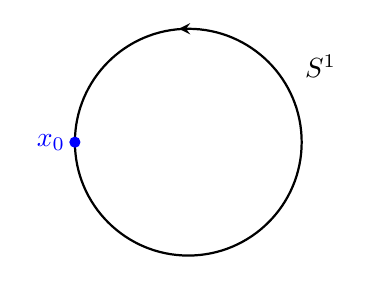
\begin{tikzpicture}[scale=1.2]
        \draw[thick] (0,0) circle (1.2cm);
        \draw[thick, ->, >=stealth] (0.1, 1.2) -- (-0.1, 1.2);
        \node at (1.4, 0.8) {$S^1$};
        \filldraw[blue] (-1.2,0) circle (1.5pt) node[left] {$x_0$};
    \end{tikzpicture}
    \caption{Lazo generatore $\sigma$ su $S^1$ con orientamento antiorario.}
\end{figure}

Le classi di omotopia distinte in $\Pi_1(S^1, x_0)$ corrispondono al numero di giri compiuti dal cappio:
\[
[c_{x_0}], \quad [\sigma], \quad [\sigma^{-1}], \quad [\sigma * \sigma] = [\sigma]^2, \quad \dots
\]
(Questa \`e solo l'intuizione; la dimostrazione rigorosa segue dal teorema di Seifert--Van Kampen, pi\`u avanti.) Pertanto, il gruppo fondamentale di $S^1$ è generato dall'unica classe $[\sigma]$ ed è isomorfo al gruppo libero $F_1$:
\[
\Pi_1(S^1, x_0) = \left\{ [\sigma]^k \;\middle|\; k \in \mathbb{Z} \right\} \cong F_1 \cong \mathbb{Z}
\]
\end{ejemplo}

\begin{ejemplo}[Gruppo fondamentale dell'unione di due circonferenze tangenti $S^1 \vee S^1$]
Consideriamo lo spazio $X = S^1 \vee S^1$ formato da due circonferenze tangenti esternamente in un punto base $x_0$.
Siano $\sigma$ e $\tau$ i due cappi orientati in senso antiorario su ciascuna delle due circonferenze.

\begin{figure}[H]
    \centering
    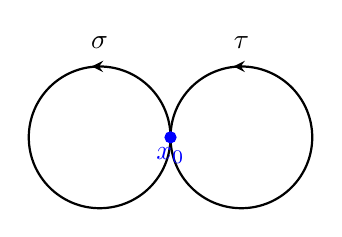
\begin{tikzpicture}[scale=1.0]
        \draw[thick] (-0.9,0) circle (0.9cm);
        \draw[thick] (0.9,0) circle (0.9cm);
        \filldraw[blue] (0,0) circle (2pt) node[below] {$x_0$};
        
        \draw[thick, ->, >=stealth] (-0.9, 0.9) -- (-1.0, 0.9);
        \node at (-0.9, 1.2) {$\sigma$};
        
        \draw[thick, ->, >=stealth] (0.9, 0.9) -- (0.8, 0.9);
        \node at (0.9, 1.2) {$\tau$};
    \end{tikzpicture}
    \caption{Rosa a due foglie $X = S^1 \vee S^1$ con i cappi generatori $\sigma$ e $\tau$.}
\end{figure}

In $\Pi_1(X, x_0)$, le concatenazioni di $\sigma$ e $\tau$ generano classi distinte a due a due:
\[
[c_{x_0}], \quad [\sigma], \quad [\tau], \quad [\sigma]^k, \quad [\tau]^h, \quad [\sigma * \tau], \quad [\tau * \sigma], \quad [\sigma * \tau^{-1}], \quad \dots
\]
Le classi di equivalenza sono le parole ridotte del tipo $[\sigma]^{k_1} [\tau]^{h_1} \cdots [\sigma]^{k_r} [\tau]^{h_r}$ con $k_i, h_i \in \mathbb{Z}$.
Di conseguenza, il gruppo fondamentale non è abeliano ed è isomorfo al gruppo libero su due generatori:
\[
\Pi_1(S^1 \vee S^1, x_0) \cong F_2
\]

Generalizzando a una rosa di $m$ circonferenze $X_m = \bigvee_{i=1}^m \mathscr{C}_i$, si ottiene:
\[
\Pi_1(X_m) \cong F_m
\]
\end{ejemplo}

\vspace{1.5em}


\section{Teoremi di Seifert-Van Kampen}

\begin{teo}[\textbf{I Teorema di Seifert-Van Kampen}]
Siano $X$ uno spazio topologico connesso per archi, $U, V \subseteq X$ aperti connessi per archi tali che $X = U \cup V$, e sia $W = U \cap V$ connesso per archi.

Consideriamo le inclusioni $i_1: W \hookrightarrow U$ e $i_2: W \hookrightarrow V$, e i rispettivi omomorfismi indotti $i_{1*}: \Pi_1(W) \to \Pi_1(U)$ e $i_{2*}: \Pi_1(W) \to \Pi_1(V)$.

Sia $N$ il più piccolo sottogruppo normale di $\Pi_1(U) * \Pi_1(V)$ contenente l'insieme di elementi del tipo:
\[
\left\{ (i_{1*}([\sigma]))^{-1} \cdot i_{2*}([\sigma]) \;\middle|\; [\sigma] \in \Pi_1(W) \right\}
\]
Allora il gruppo fondamentale di $X$ è dato dal quoziente:
\[
\Pi_1(X) \cong \frac{\Pi_1(U) * \Pi_1(V)}{N}
\]
\end{teo}

\begin{coro}
Nelle ipotesi del I Teorema di Seifert-Van Kampen, se in più l'intersezione $W = U \cap V$ è \textbf{semplicemente connessa} ($\Pi_1(W) = 0$), allora:
\[
\Pi_1(X) \cong \Pi_1(U) * \Pi_1(V)
\]
\end{coro}

\begin{coro}
Per ogni $n \geqslant 2$, la sfera $n$-dimensionale $S^n$ è semplicemente connessa:
\[
\Pi_1(S^n) = 0
\]
\end{coro}

\begin{proof}
Siano $p, q \in S^n$ con $p \neq q$. Definiamo gli aperti $U = S^n \setminus \{p\}$ e $V = S^n \setminus \{q\}$.
Allora $X = U \cup V$ e $W = U \cap V = S^n \setminus \{p,q\}$.

Gli aperti $U$ e $V$ sono omeomorfi a $\mathbb{R}^n$, quindi sono contrattili e semplicemente connessi ($\Pi_1(U) = \Pi_1(V) = 0$). Inoltre, per $n \geqslant 2$, $W \cong \mathbb{R}^n \setminus \{\bar{0}\} \simeq S^{n-1}$ è connesso per archi.

Applicando il I Teorema di Seifert-Van Kampen:
\[
\Pi_1(S^n) \cong \frac{\Pi_1(U) * \Pi_1(V)}{N} \cong \frac{0 * 0}{N} = 0
\]
\end{proof}

\begin{notacion}[\textbf{AVVISO PER L'ESAME}]
\textit{Se alla prova d'esame si richiede la dimostrazione che $S^n$ è semplicemente connessa per $n \geqslant 2$, occorre riportare la dimostrazione diretta dettagliata con il Lemma del numero di Lebesgue (del 06/10/2026)}.
\end{notacion}

\vspace{1.5em}

\begin{teo}[\textbf{II Teorema di Seifert-Van Kampen}]
Siano $X$ uno spazio topologico connesso per archi, $U, V \subseteq X$ aperti connessi per archi tali che $X = U \cup V$, e supponiamo che l'intersezione $W = U \cap V$ sia l'unione disgiunta di due aperti semplicemente connessi.

Se $V$ è semplicemente connesso, allora:
\[
\Pi_1(X) \cong \Pi_1(U) * \mathbb{Z}
\]
\end{teo}

\begin{coro}
$\Pi_1(S^1) \cong \mathbb{Z}$.
\end{coro}

\begin{proof}
Siano $p, q \in S^1$ due punti distinti ($p \neq q$). Definiamo $U = S^1 \setminus \{p\}$ e $V = S^1 \setminus \{q\}$.
Allora $S^1 = U \cup V$ e l'intersezione $W = U \cap V = S^1 \setminus \{p, q\}$ è l'unione disgiunta di due intervalli aperti (ciascuno semplice connesso e connesso per archi).

\begin{figure}[H]
    \centering
    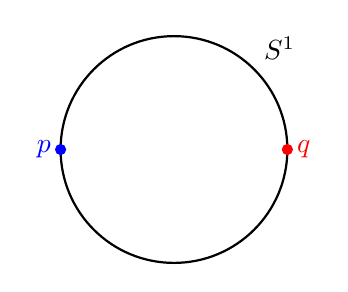
\begin{tikzpicture}[scale=1.2]
        \draw[thick] (0,0) circle (1.2cm);
        \node[above right] at (0.85, 0.85) {$S^1$};
        \filldraw[blue] (-1.2, 0) circle (1.5pt) node[left] {$p$};
        \filldraw[red] (1.2, 0) circle (1.5pt) node[right] {$q$};
    \end{tikzpicture}
    \caption{Decomposizione di $S^1$ in due aperti $U, V$ con intersezione $W$ disgiunta.}
\end{figure}

Inoltre $U \cong V \cong \mathbb{R}$ sono connessi per archi e $V$ \`e semplicemente connesso ($\Pi_1(V) = 0$).
Dal II Teorema di Seifert-Van Kampen segue direttamente:
\[
\Pi_1(S^1) = \Pi_1(U) * \mathbb{Z} = 0 * \mathbb{Z} = \mathbb{Z}
\]
\end{proof}

\vspace{1.5em}

\begin{lema}
Siano $X$ uno spazio topologico, $x_0 \in X$ e $J$ un arco aperto, cio\`e un sottospazio $J \cong\ ]-1,1[$ tramite un omeomorfismo $\psi: J \to\ ]-1,1[$ con $\psi(x_0) = 0$ (quindi $x_0 \in J$). Posto $Y = X \cup J$, supponiamo $X \cap J = \{x_0\}$ e che $X$ e $J$ siano chiusi in $Y$.
Allora $X$ \`e un \textbf{retratto di deformazione} di $Y$ e, di conseguenza, l'inclusione induce un isomorfismo
\[
\Pi_1(X, x_0) \cong \Pi_1(X \cup J, x_0).
\]
\end{lema}

\begin{proof}
Sia $r: Y \to X$ definita da $r(y) = y$ su $X$ e $r(y) = x_0$ su $J$. Sono compatibili su $X \cap J = \{x_0\}$, e $X, J$ sono chiusi: per il Lemma di Incollamento $r$ \`e continua. Chiaramente $r \circ i = \mathrm{Id}_X$.

Definiamo $H: Y \times I \to Y$ ponendo $H(y,s) = y$ se $y \in X$, e $H(y,s) = \psi^{-1}\big((1-s)\,\psi(y)\big)$ se $y \in J$. Sulla intersezione $X \cap J$ si ha $H(x_0, s) = \psi^{-1}(0) = x_0$ in entrambe le definizioni, quindi $H$ \`e continua (Lemma di Incollamento su $X \times I$ e $J \times I$, chiusi). Inoltre $H(y,0) = y = \mathrm{Id}_Y(y)$ e $H(y,1) = r(y) = (i\circ r)(y)$. Dunque $\mathrm{Id}_Y \simeq i \circ r$, cio\`e $X$ \`e un retratto di deformazione di $Y$ (e $H$ fissa $X$ puntualmente). Per l'invarianza omotopica del gruppo fondamentale, $i_*: \Pi_1(X,x_0) \to \Pi_1(Y,x_0)$ \`e un isomorfismo\hfill$\square$
\end{proof}

\begin{observacion}[Nota di correzione]
Negli appunti originali il lemma era enunciato con ``$I'$ intervallo aperto di $\mathbb{R}^n$'' e la omotopia scritta come $(1-s)y + s\,r(y)$; ma nell'applicazione alla rosa a foglie $I'$ \`e un \emph{arco di circonferenza}, per il quale il segmento retto non resta in $Y$. La versione qui sopra (con l'omeomorfismo $\psi$) \`e quella che si applica correttamente.
\end{observacion}

\vspace{1.5em}
\begin{coro}
Sia $X_n = \bigcup_{i=1}^n \mathscr{C}_i$ la rosa a $n$ foglie (unione puntata di $n$ circonferenze). Allora:
\[
\Pi_1(X_n) \cong F_n \quad (\text{gruppo libero su } n \text{ generatori})
\]
\end{coro}

\begin{proof}
Procediamo per induzione su $n \geqslant 1$:
\begin{figure}[H]
    \centering
    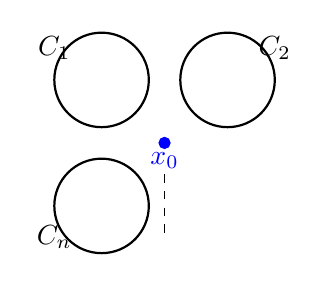
\begin{tikzpicture}[scale=1.0]
        % Rosa a 3 foglie
        \draw[thick] (-0.8,0.8) circle (0.6cm);
        \draw[thick] (0.8,0.8) circle (0.6cm);
        \draw[thick] (-0.8,-0.8) circle (0.6cm);
        \filldraw[blue] (0,0) circle (2pt) node[below] {$x_0$};
        \node at (-1.4,1.2) {$\mathscr{C}_1$};
        \node at (1.4,1.2) {$\mathscr{C}_2$};
        \node at (-1.4,-1.2) {$\mathscr{C}_n$};
        \draw[dashed] (0,-0.4) -- (0,-1.2);
    \end{tikzpicture}
    \caption{Rosa a $n$ foglie $X_n$.}
\end{figure}

Per $n=1$, $X_1 = S^1 \implies \Pi_1(X_1) \cong \mathbb{Z} = F_1$.
Assumiamo il risultato vero per $n-1$. Fissiamo $q \in \mathscr{C}_n \setminus \{x_0\}$ e poniamo $U = X_n \setminus \{q\}$, $V = \mathscr{C}_n \setminus \{x_0\}$.
Allora $U$ e $V$ sono aperti in $X_n$, $X_n = U \cup V$ e $W = U \cap V = \mathscr{C}_n \setminus \{q, x_0\}$ è un'unione disgiunta di due aperti semplicemente connessi.

$V$ è un intervallo aperto, quindi semplicemente connesso.
Inoltre $U = X_{n-1} \cup J$, dove $J = \mathscr{C}_n \setminus \{q\}$ \`e un arco aperto che interseca $X_{n-1}$ solo in $x_0$ (entrambi sono chiusi in $U$: $X_{n-1}$ \`e compatto, e $J$ \`e chiuso in $U$ perch\'e $\overline{J} = \mathscr{C}_n$ incontra $X_{n-1}$ solo in $x_0 \in J$). Quindi $X_{n-1}$ \`e un retratto di deformazione di $U$.
Per il Lemma precedente, $\Pi_1(U) \cong \Pi_1(X_{n-1})$.

Sfruttando il II Teorema di Seifert-Van Kampen:
\[
\Pi_1(X_n) = \Pi_1(U) * \mathbb{Z} = \Pi_1(X_{n-1}) * \mathbb{Z} \cong F_{n-1} * \mathbb{Z} = F_n
\]
\end{proof}
\vspace{1.5em}

\begin{ejercicio*}
Calcolare il gruppo fondamentale dello spazio $X = \mathbb{R}^3 \setminus S^1$.

\begin{proof}[Svolgimento]
Rappresentiamo $S^1$ nel piano $z=0$ come $S^1 = \{(x,y,z) \in \mathbb{R}^3 \mid z=0, \, x^2+y^2=1\}$.
Consideriamo il disco chiuso $\overline{B^2} = \{(x,y,z) \in \mathbb{R}^3 \mid z=0, \, x^2+y^2 \leqslant 1\}$.

Decomponiamo $X = \mathbb{R}^3 \setminus S^1$ nell'unione di due aperti $U$ e $V$:
\begin{itemize}
    \item $U = \mathbb{R}^3 \setminus \overline{B^2}$ è un aperto semplicemente connesso ($\Pi_1(U) = 0$): intuitivamente, il disco chiuso si pu\`o ``schiacciare'' in un punto, per cui $U$ ha lo stesso tipo di omotopia di $\mathbb{R}^3 \setminus \{\text{pt}\} \simeq S^2$, che \`e semplicemente connessa.
    \item $V = \{(x,y,z) \in \mathbb{R}^3 \mid x^2+y^2 < 1\}$ (la parte interna di un cilindro infinito attorno all'asse $z$ con direttrice $S^1$). $V$ è contrattile, quindi semplicemente connesso ($\Pi_1(V) = 0$).
\end{itemize}

L'intersezione $W = U \cap V$ si scompone nell'unione disgiunta di due aperti semplicemente connessi:
\[
A_1 = \left\{(x,y,z) \in \mathbb{R}^3 \;\middle|\; z > 0, \, x^2+y^2 < 1\right\}
\]
\[
A_2 = \left\{(x,y,z) \in \mathbb{R}^3 \;\middle|\; z < 0, \, x^2+y^2 < 1\right\}
\]

\begin{figure}[H]
    \centering
    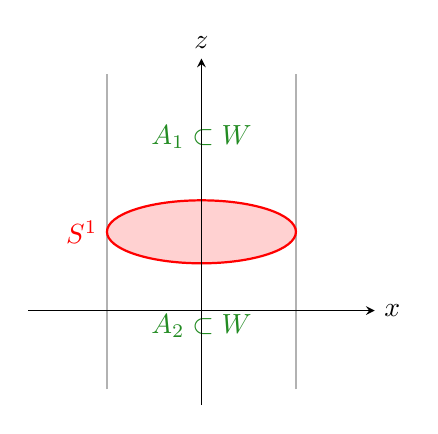
\begin{tikzpicture}[scale=1.0]
        % Cilindro V
        \draw[thick, gray!60] (-1.2,-2) -- (-1.2,2);
        \draw[thick, gray!60] (1.2,-2) -- (1.2,2);
        
        % Disco B^2
        \fill[red!30, opacity=0.6] (0,0) ellipse (1.2cm and 0.4cm);
        \draw[thick, red] (0,0) ellipse (1.2cm and 0.4cm);
        \node[red, left] at (-1.2,0) {$S^1$};

        % Regioni A_1 y A_2
        \node[ForestGreen] at (0,1.2) {$A_1 \subset W$};
        \node[ForestGreen] at (0,-1.2) {$A_2 \subset W$};

        % Ejes
        \draw[->, >=stealth] (-2.2,-1) -- (2.2,-1) node[right] {$x$};
        \draw[->, >=stealth] (0,-2.2) -- (0,2.2) node[above] {$z$};
    \end{tikzpicture}
    \caption{Decomposizione dello spazio $X = \mathbb{R}^3 \setminus S^1$ per l'applicazione di Seifert-Van Kampen.}
\end{figure}

Siamo nelle ipotesi del II Teorema di Seifert-Van Kampen:
\[
\Pi_1(\mathbb{R}^3 \setminus S^1) \cong \Pi_1(U) * \mathbb{Z} = 0 * \mathbb{Z} = \mathbb{Z}
\]
\end{proof}
\end{ejercicio*}

\vspace{2em}



\section{Applicazioni ed Esempi del Gruppo Fondamentale}

\begin{lema}
La circonferenza $S^1 = \partial B^2$ \textbf{non è un retratto} del disco chiuso $B^2$.
\end{lema}

\begin{proof}
Supponiamo per assurdo che esista una retrazione $r: B^2 \to S^1$, ossia un'applicazione continua tale che $r \circ i = \mathrm{Id}_{S^1}$, dove $i: S^1 \hookrightarrow B^2$ è l'inclusione canonica.

Passando agli omomorfismi indotti sul gruppo fondamentale:
\begin{tikzcd}[scale=1.2]
    \Pi_1(S^1) \arrow[r, "i_*"] \arrow[rr, bend right=30, "(\mathrm{Id}_{S^1})_*"'] & \Pi_1(B^2) \arrow[r, "r_*"] & \Pi_1(S^1)
\end{tikzcd}

Si ha che $(r \circ i)_* = r_* \circ i_* = (\mathrm{Id}_{S^1})_* = \mathrm{Id}_{\Pi_1(S^1)}$.
Sostituendo i gruppi fondamentali noti ($\Pi_1(S^1) \cong \mathbb{Z}$ e $\Pi_1(B^2) = 0$ in quanto $B^2$ è convesso):
\[
\Pi_1(S^1) = \mathrm{Id}_*(\Pi_1(S^1)) = r_*(i_*(\Pi_1(S^1))) \subseteq r_*(\Pi_1(B^2)) = r_*(0) = 0
\]
Otteniamo quindi che $\mathbb{Z} = 0$, il che è una palese contraddizione\hfill$\square$
\end{proof}

\vspace{1.5em}

\begin{teo}[Teorema del Punto Fisso di Brouwer in dimensione 2]
Ogni applicazione continua $f: B^2 \to B^2$ ammette almeno un punto fisso, ossia esiste $\bar{x} \in B^2$ tale che $f(\bar{x}) = \bar{x}$.
\end{teo}

\begin{proof}
Supponiamo per assurdo che $f(x) \neq x$ per ogni $x \in B^2$.
Possiamo allora definire un'applicazione $r: B^2 \to \partial B^2 = S^1$ costruita geometricamente come segue: per ogni $x \in B^2$, si considera la semiretta uscente da $f(x)$ e passante per $x$, e si definisce $r(x)$ come il punto di intersezione di tale semiretta con la circonferenza di bordo $S^1$.

\begin{figure}[H]
    \centering
    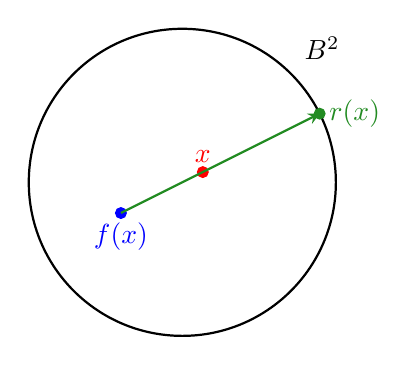
\begin{tikzpicture}[scale=1.3]
        % Disco B^2
        \draw[thick] (0,0) circle (1.5cm);
        \node[above right] at (1.1,1.1) {$B^2$};
        
        % Punti f(x) e x
        \filldraw[blue] (-0.6, -0.3) circle (1.5pt) node[below] {$f(x)$};
        \filldraw[red] (0.2, 0.1) circle (1.5pt) node[above] {$x$};
        
        % Semiretta e intersezione r(x)
        \draw[thick, ForestGreen, ->, >=stealth] (-0.6,-0.3) -- (1.3416, 0.6708);
        \filldraw[ForestGreen] (1.3416, 0.6708) circle (1.5pt) node[right] {$r(x)$};
    \end{tikzpicture}
    \caption{Costruzione della retrazione $r(x)$ a partire da una mappa priva di punti fissi.}
\end{figure}

L'applicazione $r$ così definita è continua. Per verificarlo esplicitamente, posto $u = x - f(x) \neq \bar{0}$, il punto $r(x) = x + \lambda(x)\,u$ \`e quello con $\lambda \geqslant 0$ tale che $\|x + \lambda u\|^2 = 1$, cio\`e $\|u\|^2\lambda^2 + 2\langle x,u\rangle \lambda + \|x\|^2 - 1 = 0$, e quindi
\[
\lambda(x) = \frac{-\langle x,u\rangle + \sqrt{\langle x,u\rangle^2 + \|u\|^2\,(1-\|x\|^2)}}{\|u\|^2},
\]
che \`e continua in $x$ (il discriminante \`e $\geqslant 0$ perch\'e $\|x\| \leqslant 1$, e $u \neq \bar 0$). Se $\|x\| = 1$ si ha $\langle x, u\rangle = 1 - \langle x, f(x)\rangle \geqslant 0$ (perch\'e $\|f(x)\| \leqslant 1$), quindi $\lambda(x) = 0$ e $r(x) = x$. Come visto sopra, $r(x) = x$ per ogni $x \in S^1 = \partial B^2$ (il punto $x$ giace gi\`a sul bordo).

Pertanto $r: B^2 \to S^1$ sarebbe una retrazione continua dal disco chiuso alla sua circonferenza di bordo. Ma questo contraddice il Lemma precedente, che stabilisce che $S^1$ non è un retratto di $B^2$.
Di conseguenza, deve esistere almeno un punto fisso $\bar{x} \in B^2$ tale che $f(\bar{x}) = \bar{x}$\hfill$\square$
\end{proof}

\vspace{2em}


\section{Gruppo Fondamentale del Toro Privato di un Punto}

\begin{prop}
Sia $T^2 = S^1 \times S^1$ il toro bidimensionale e $p \in T^2$.
Il gruppo fondamentale del toro privato di un punto è il gruppo libero su due generatori:
\[
\Pi_1(T^2 \setminus \{p\}) \cong F_2
\]
\end{prop}

\begin{proof}
Rappresentiamo il toro come il quoziente del quadrato unitario $T^2 = Q / \sim$, dove $Q = [0,1] \times [0,1]$ e la relazione di equivalenza identifica i lati opposti.
Sia $p \in \mathring{Q}$ un punto interno del quadrato (la scelta di $p$ \`e irrilevante: le traslazioni di $T^2$ sono omeomorfismi e agiscono transitivamente sui punti).

Consideriamo la proiezione radiale dal punto $p$ verso il bordo $\partial Q$:
\Func{r}{Q \setminus \{p\}}{\partial Q}{x}{\text{punto di intersezione della semiretta uscente da } p \text{ passante per } x \text{ con } \partial Q}

\begin{figure}[H]
    \centering
    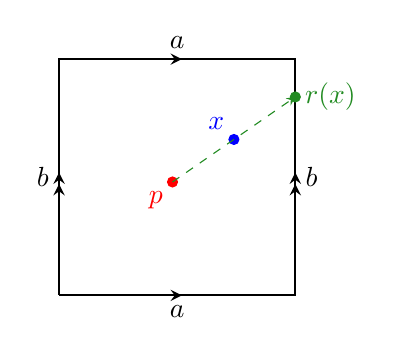
\begin{tikzpicture}[scale=1.2]
        % Cuadrado Q
        \draw[thick] (0,0) -- (2.5,0) node[midway, below] {$a$} -- (2.5,2.5) node[midway, right] {$b$} -- (0,2.5) node[midway, above] {$a$} -- (0,0) node[midway, left] {$b$};
        
        % Flechas de identificación de lados
        \draw[thick, ->, >=stealth] (1.1,0) -- (1.3,0);
        \draw[thick, ->, >=stealth] (1.1,2.5) -- (1.3,2.5);
        \draw[thick, ->>, >=stealth] (0,1.1) -- (0,1.3);
        \draw[thick, ->>, >=stealth] (2.5,1.1) -- (2.5,1.3);

        % Punto p interno y proyectado
        \filldraw[red] (1.2, 1.2) circle (1.5pt) node[below left] {$p$};
        \filldraw[blue] (1.85, 1.65) circle (1.5pt) node[above left] {$x$};
        \draw[dashed, ForestGreen, ->, >=stealth] (1.2,1.2) -- (2.5, 2.1);
        \filldraw[ForestGreen] (2.5,2.1) circle (1.5pt) node[right] {$r(x)$};
    \end{tikzpicture}
    \caption{Proiezione radiale $r: Q \setminus \{p\} \to \partial Q$.}
\end{figure}

L'applicazione $r$ è ben definita e continua.
Inoltre, per ogni $x \in \partial Q$ si ha $r(x) = x$, quindi $r$ è una retrazione di $Q \setminus \{p\}$ su $\partial Q$.

Costruiamo la seguente omotopia $H: (Q \setminus \{p\}) \times I \to Q \setminus \{p\}$ data da:
\[
H(x, s) = (1-s)x + s\, r(x)
\]
$H$ \`e continua (e ha valori in $Q \setminus \{p\}$: il segmento da $x$ a $r(x)$ giace sulla semiretta uscente da $p$ che passa per $x$, quindi non contiene $p$; inoltre $Q$ \`e convesso) e soddisfa $H(x,0) = x = \mathrm{Id}_{Q \setminus \{p\}}(x)$ e $H(x,1) = r(x) = (i \circ r)(x)$.
Ciò prova che $\partial Q$ è un \textbf{retratto di deformazione} di $Q \setminus \{p\}$.

Poich\'e $H$ lascia fisso ogni punto di $\partial Q$, \`e compatibile con le identificazioni dei lati opposti, quindi passa al quoziente (si usa che $\pi \times \mathrm{Id}_I$ \`e ancora una applicazione quoziente, perch\'e $I$ \`e localmente compatto). Si ottiene una omotopia $\widetilde{H}$ su $T^2 \setminus \{p\} = (Q \setminus \{p\})/\!\sim$ e una retrazione
\[
\widetilde{r}: T^2 \setminus \{p\} \longrightarrow \partial Q / \sim ,
\]
cio\`e $\partial Q/\!\sim$ \`e un retratto di deformazione del toro bucato.

Nel quoziente i quattro lati si identificano a due a due (lato $a$ con lato $a$, lato $b$ con lato $b$) e i quattro vertici diventano un unico punto: $\partial Q / \sim$ \`e quindi formato da due circonferenze ($a$ e $b$) incollate in un punto, ossia la rosa a due foglie $S^1 \vee S^1$.

Sfruttando l'invarianza omotopica del gruppo fondamentale:
\[
\Pi_1(T^2 \setminus \{p\}) \cong \Pi_1(\partial Q / \sim) \cong \Pi_1(S^1 \vee S^1) \cong F_2
\]
\end{proof}

\vspace{2em}

